\chapter{A search for new physics in events with a Z boson, missing transverse energy, and jets}

\section{Motivations}

  This is some great motivation!

  \subsection{Motivating Models} \label{sec:susy_models}

  GMSB: https://arxiv.org/pdf/hep-ph/9707450.pdf
  https://arxiv.org/pdf/hep-ph/9801271.pdf

  \begin{figure}[h!]
    \centering
    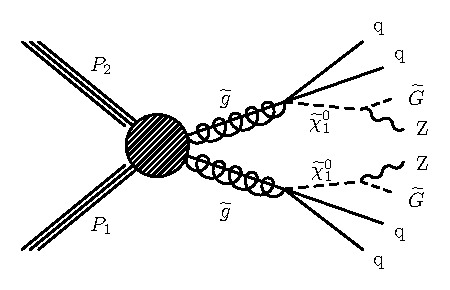
\includegraphics[width=.5\textwidth]{figures/diagrams/T5ZZ.pdf}
    \caption{The Feynman diagram for the additional term added to The Standard Model lagrangian to produce the simplified supersymmetric model used to interpret this in analysis in the context of ``strong SUSY". In this model, SUSY is broken by the Gauge sector (wtf is GMSB) }
    \label{fig:feynman_str}
  \end{figure}

  \begin{figure}
  \begin{center}
    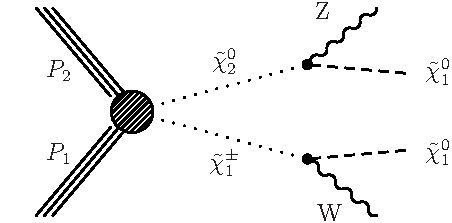
\includegraphics[width=0.3\textwidth]{figures/diagrams/TChiWZ.pdf} 
    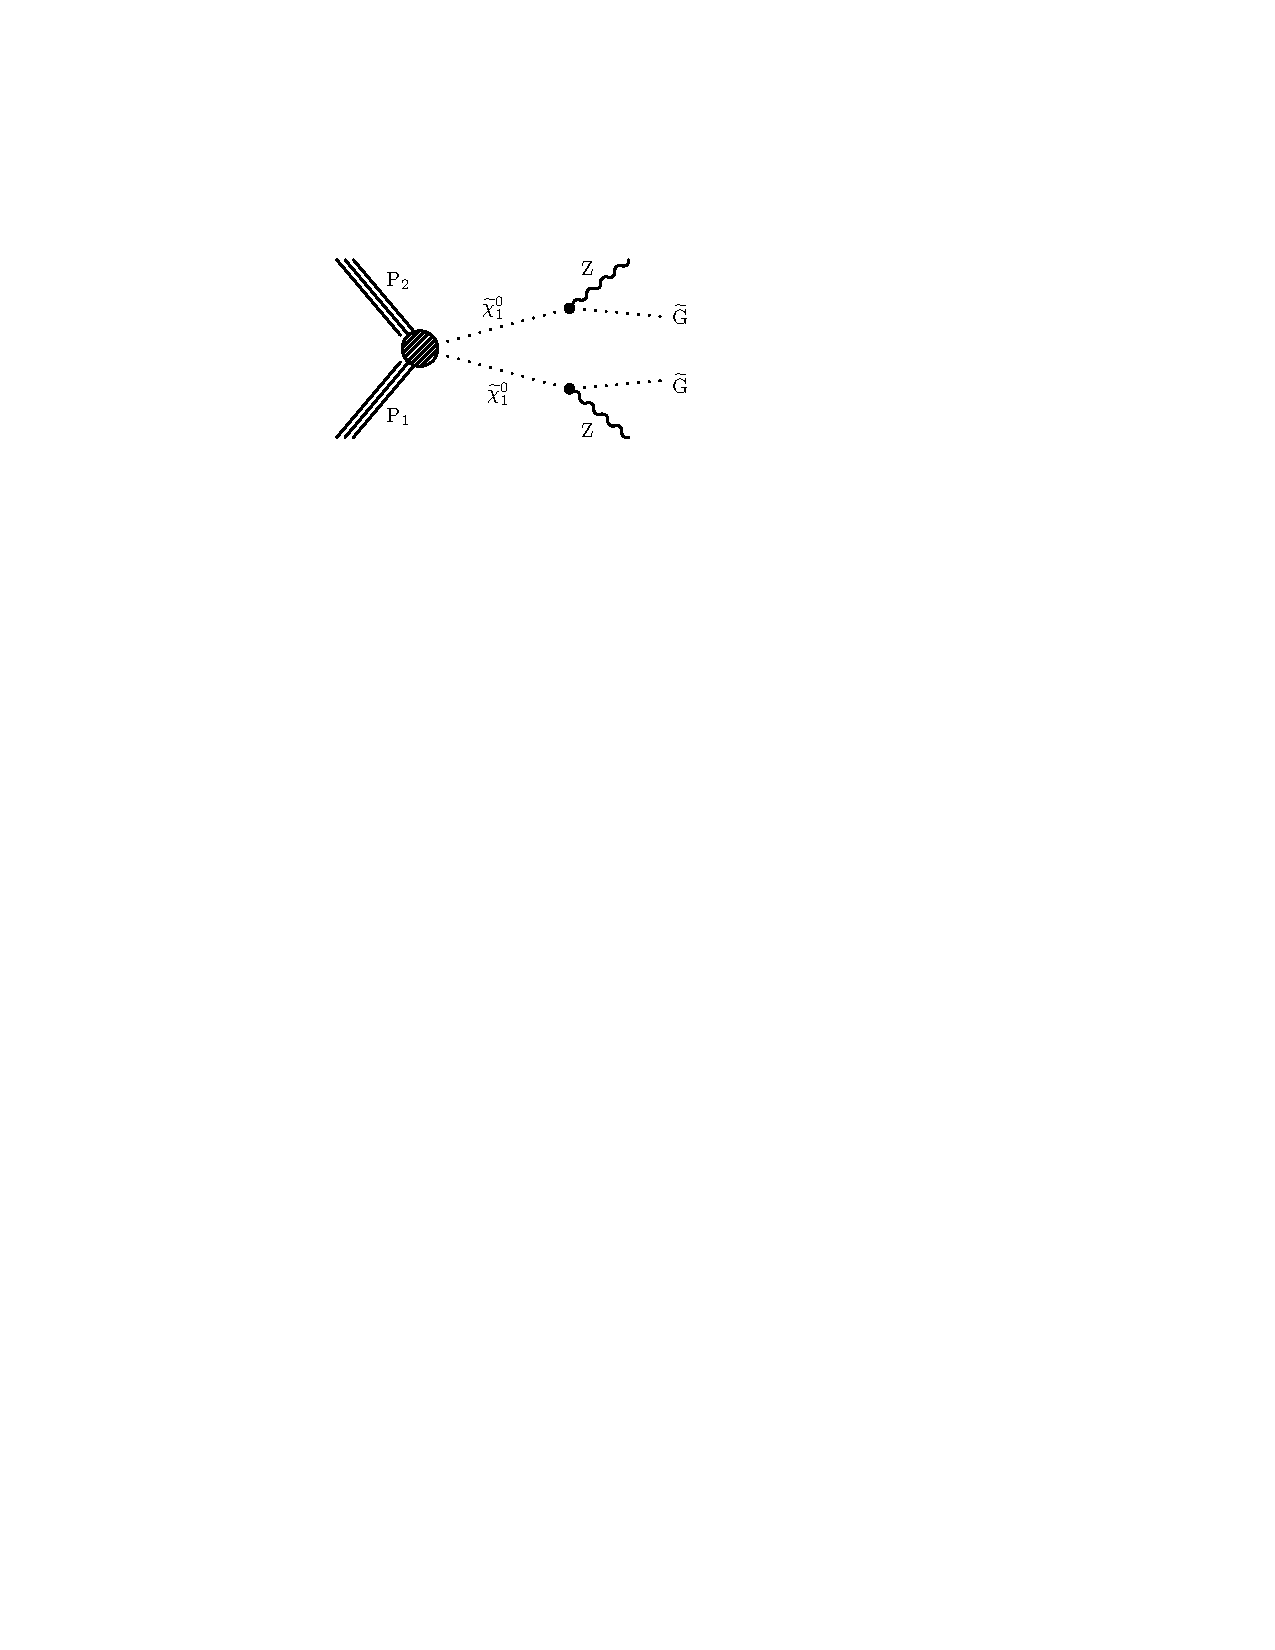
\includegraphics[width=0.3\textwidth]{figures/diagrams/TChiZZ.pdf} 
    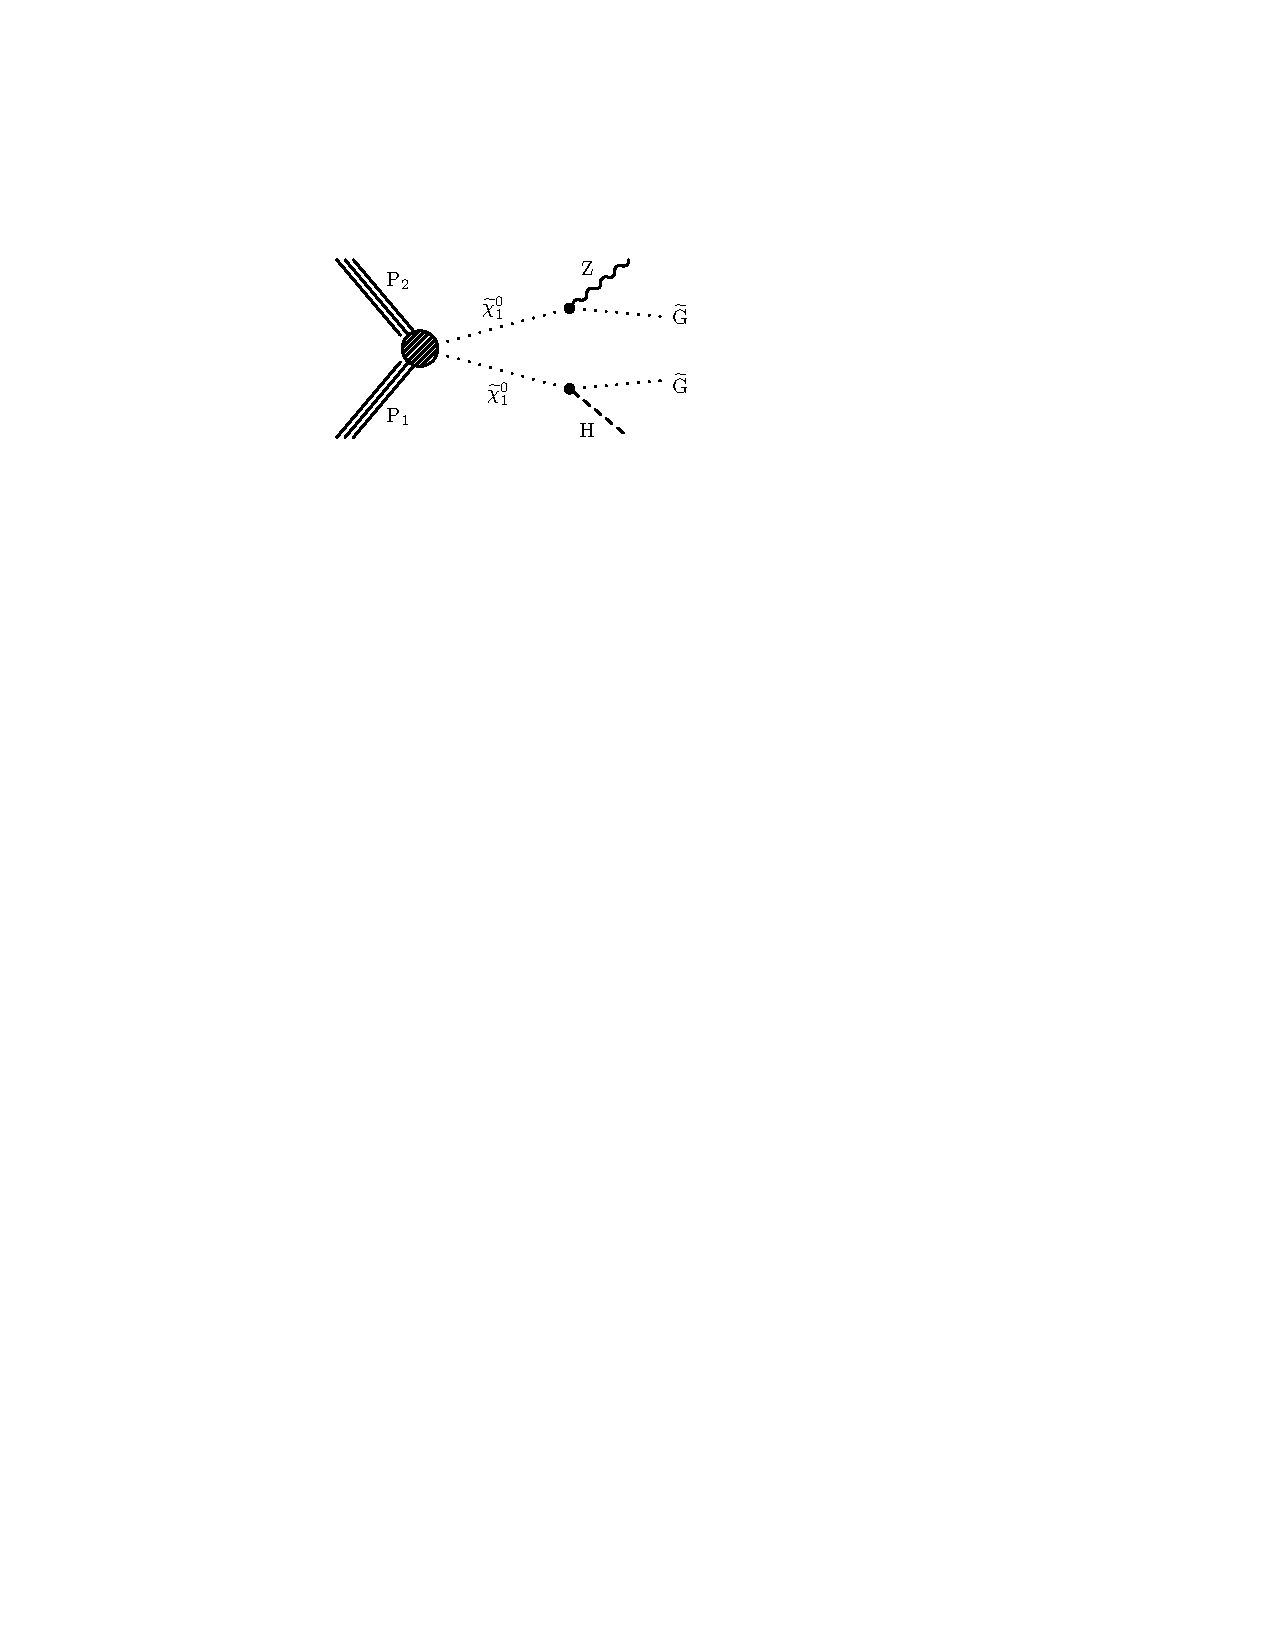
\includegraphics[width=0.3\textwidth]{figures/diagrams/TChiHZ.pdf} 
  \end{center}
  \caption{
    \label{sig:feynman_ewk} \todo{same cap as AN}
    Diagrams for models with electroweak production.
    The left shows chargino-neutralino production decaying to WZ+\MET (TChiWZ).
    The middle shows neutralino-neutralino production decaying to ZZ+\MET (TChiZZ),
    while the right shows the same production decaying to HZ+\MET (TChiHZ).
    The TChiZZ and TChiHZ diagrams containing a massless gravitino ($\tilde{\mathrm{G}}$) represent gauge mediated SUSY breaking (GMSB) models.
  }
\end{figure}

  1. Show the models Strong and EWK SUSY model diagrams we use here.
  2. Discuss why they are useful tools (i.e. give an idea of SMS)

  \subsection{SUSY Simulation} \label{sec:susy_simulation}
    Explain how madgraph is used here, what crap we assume, ect...

\section{Analysis Strategy}

  \subsection{Background Considerations}

    \subsubsection{Leptonic Final States} \label{sec:leptonic_final_states}
      The Z boson can decay to any fermion. In theory, one could perform this analysis in an all hadronic final state, which might seem advantageous as the Z will decay to hadrons approximately 10 times as often as it will decay to light leptons. \todo{Add some figure for the Z decay rates, probably can site the PDG}. However, there are several reasons leptonic final states are highly advantageous.

      In hadron colliders, the most common types of final states are those with only hadronic activity, as can be seen in figure \ref{fig:lhc_decay_modes}; leptonic final states provide a much cleaner population in which to search for Z bosons. Additionally, as referenced in \ref{sec:electron_measurement_pipeline}, \ref{sec:muon_measurement_pipeline}, and \ref{sec:MET_reco}, the fidelity of energy measurements for the light leptons is much better than for jets at CMS. This provides great advantage for background discrimination; leptons from Z boson decays will tend to have a very specific dilepton mass, a quantity reconstructed from the momentum measurements.

      The decays of the Z produce two opposite sign, same flavor fermions. A further benefit of the leptonic channel is that flavor and charge identification is fairly easy for the light leptons but nearly impossible to identify for jets at the current state of the art (for instance, one can not say with high confidence that a jet was produced by a positively charged charm quark). Finally, the energy and momentum measurements for the light leptons are much better than for jets because of the complexity involved in making good energy measurements for jets. \todo{Point to some discussion about hadron calorimetry, the basic idea here is just that jets have neutral particles and their contribution to the energy measurement needs to be implied by the reconstruction algorithm} 

      Therefore, even though the decay rate to light leptons from Z bosons is lower than the production rate to hadronic final states, the better energy resolution and lower background rate makes the leptonic final state far more powerful.

      When using the leptonic final states, there are essentially two other background sources of leptons we must consider, these are $\gamma$ and W decays. The W boson will decay into leptons only with a complimentary neutrino, this means that in order to select a pair of opposite charge and same flavor leptons, there must be at least two W bosons in the event. Because the decays of the W will be independent, there is only a 50\% chance that the two leptons in an event where two Ws decay leptonically will have the same flavor. As will be discussed later, this makes the background prediction for these types of events very easy as events with two same flavor leptons can be used to model essentially any kinematical distribution.

      Depending on the source of the Ws, the kinematics of the leptons will differ. However, a general rule is that the total energy in the event will be peaked at some low value, near the threshold to produce the event, essentially the sum of the mass of all the prompt particles, and decay exponentially from there. Many kinematic distributions are highly correlated with the total energy in the event. In the case of the Z decay, we know the dilepton mass distribution will not be correlated

      It turns out the most common source of W bosons is through the production of two top quarks, which decay to a bottom quark and a W Boson. To reject these events, we will use B-tagging, described in \todo{add reference to b-tagging section}. Further, the dilepton mass in these events will be essentially random \todo{Add a figure of WW and TTBar production MLL plot for ZMET. Is the distribution flat or falling?} but biased towards lower values. 

      less likely, whereas for Z decay, the breit-wigner distribution predisposes the dilepton mass to be near 91 GeV. 

      The overall dilepton mass distribution will be a falling distribution with a small bump for the Z Boson. 

      \todo{Need to close this off with a discussion about how the backgrounds are mainly DY, TTBar, and VZ}

      Finally, due to the instability of the $\tau$ lepton, we neglect this channel from the search. $\tau$ leptons are much harder to identify than the light leptons, and further they can decay to light leptons in a flavor symmetric manner, so are predicted by that background channel's prediction method.

    \subsubsection{Hadronic Activity Requirements}
      As mentioned above, the major production mode of opposite sign dilepton pairs with dilepton mass near 91 GeV is from Drell-Yan production of Z. The diagram for this type of process is shown in \ref{fig:DY-diagram}. As can be seen in the figure, the leading order diagram for this process has no free quarks or gluons. That there are no free colored particles means that the vast majority of these events will likewise come without any jets. Diagrams with ISR and FSR which take a cross-section production hit of roughly 1/5 \todo{explain this}, which means that we can suppress the DY background by a factor of 100 by requiring at least 2 jets in an event. This keeps our signal count low. Further, the prediction of 0 or 1 jet bins is a completely different process due to the sources of \MET, and many of our motivating models will have many jets as part of their decay chain. 

      \begin{figure}[h!]
        \centering
        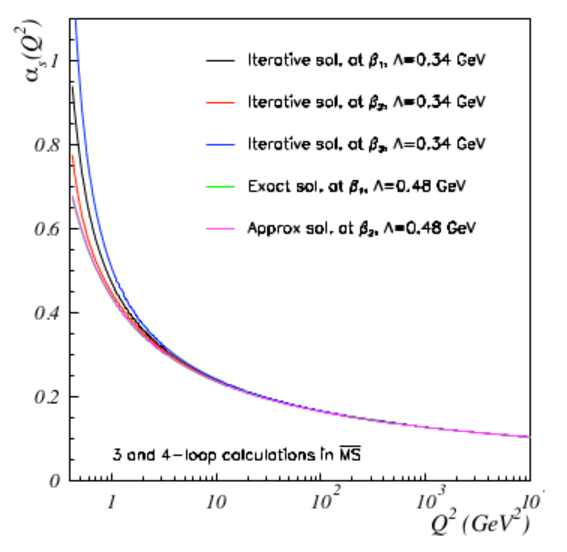
\includegraphics[width=.5\textwidth]{figures/QCD_Coupling_Running.pdf}
        \caption{The QCD coupling constant computed to different orders and different cutoff scales. The production of the Z boson is much more likely at center of mass energy near the mass of the Z. This means that $\alpha_s$ is between $\frac{1}{5}$ and $\frac{1}{10}$, which can be viewed as the zeroth order multiplicative correction to the DY with a single ISR or FSR jet cross section} 
        \label{fig:alpha_s_running}
      \end{figure}

      In fact, strongly produced SUSY models described in \ref{sec:susy_models} anticipate lots of hadronic activity. Therefore, in search regions targeted at those models, we also also ask for lots of hadronic activity by selecting events with high $H_T$, the scalar sum of transverse energy for all jets in an event, above certain thresholds. This further rejects DY events.

      \begin{figure}[h!]
        \centering
        
\includegraphics[width=.5\textwidth]{figures/placeholder.png}
        \caption{\todo{To Be Updated with DY figure.}}
        \label{fig:DY-diagram}
      \end{figure}

    \subsubsection{\MET Binning}
      Again, inspecting the diagram above, when the Z decays to charged leptons, no neutrinos are produced. This means that DY has no genuine \MET, any missing energy must come from mismeasurements of the jet energy, misattributions of jets to the DY vertex, or loss of objects out of the detectors fiducial area. These should be relatively small effects and we will discuss how we predict the \MET distribution for this type of event in the following sections. For now, consider that the leading background when searching for Z bosons can be reduced dramatically by considering only events with high \MET. In this analysis, we only look at events with more than 100 GeV of missing energy.

    \subsubsection{MT2}
      The MT2 variable is defined as

      \[
      \min\max{whatever}
      \]

      When a pair of W bosons decay into a lepton and a neutrino, we can see that this value should not be able to be larger than the mass of the W boson, since by summing over all possibilities, we will get the true values which makes the outer minimum select at most the mass of the W (there is no lower limit). However, in the case of an arbitrary decay, for instance in DY or in signal models with dark matter, there is no need for this value to be smaller than the mass of the W and generally higher values will be found. Therefore, we can use this quantity as a handle for rejecting events where the leptons come from two W bosons. We require in our signal regions that MT2 be at least greater than 80 GeV, near the mass of the W boson. This mainly rejects the TTBar background. \todo{Why does any TTBar actually get through?}

    \subsubsection{B-Tagging}
      We also like to bin in b-tags. This is because the background composition changes dramatically with b-tagging as the second largest background is TTBar. This allows us to use a slightly higher MT2 cut in regions with a b-tag, as they will be more dominated by TTBar than by DY since DY is likely not going to have a b-tag even though it might.

\section{Object Selection}

  \todo{Add all the selection variables to the glossary}

  After the particle flow algorithm identifies lepton, jet, and photon candidates, and before events can be classified as belonging to the various search, control, and closure regions, an additional set of selections are applied in order to further purify the analysis object collection. The purpose of this section is to define these selections, sometimes called a ``preselection."

  \subsection{Lepton ID}
    There are essentially two ways to get ``fake" leptons in the lepton population:

    \begin{enumerate}
      \item A set of calorimeter and tracker hits from hadronic activity mimics the geometry expected by an lepton closely enough that a lepton is reconstructed from what should be called a jet.
      \item An unstable particle, normally a charm or bottom quark, decays via a(n), often virtual, W boson and emits a real lepton and its complimentary neutrino. In physics parlance, this is called \emph{non-prompt} lepton, as it is a secondary decay (\emph{prompt} meaning created at the primary vertex).
    \end{enumerate}

    Although item (2) is a ``real" lepton in the colloquial sense, in the context of most analyses, this one included, we do not want these sorts of objects contaminating our lepton population. To guard against these fake leptons, an additional set of cuts, called an ID is required to be passed by each candidate before it is considered a ``good" lepton.

    In this analysis, we identify two ``working points" for leptons, tight and loose. These categories are defined based the lepton flavor and a set of cuts described below. Any lepton which passes the criteria to be classified as tight would necessarily pass the criteria to be classified as loose.

  \subsection{Lepton Isolation}
    In addition to the ID, isolation requirements are also necessary for leptons to be added to the analysis selection. In this analysis we use the variable miniRelIso, which is defined as the energy inside a variable size cone, determined by the lepton candidates \pt, about the lepton divided by the leptons \pt. The cone size is set by \pt in the following manner (units in \GeV):

    \[   
      \Delta R = 
      \begin{cases}
        0.2                & \pt < 50  \\
        \frac{10}{\pt}     & 50 \le \pt < 200 \\
        0.05               & \pt \ge 200 \\
      \end{cases}.
    \]

    The miniRelIso variable is then defined as the energy of all particle flow candidates inside the cone of size $\Delta R$ with effective area corrections applied \todo{cite EA corrections} divided by the \pt of the lepton.

    \[
      \text{miniRelIso} = \frac{\text{E}_\text{cone}}{\pt}.\footnote{The miniRelIso variable is normally defined as just the energy of the cone, but for the sake of simplicity in terms of the use in this analysis, we define it as the ratio of the conventional miniRelIso to the lepton's \pt}
    \]


  \subsection{Electron ID and Isolation} \label{sec:electron_id_and_isolation}
    \todo{cite https://arxiv.org/pdf/1502.02701.pdf}
    The electron candidates are required to pass the following cuts in addition to the particle flow identification:

    \begin{table}[!h]
      \begin{center}
      \caption{\label{table:electrons} Requirements for electron identification in addition to particle flow. Variables can be looked up in the \hyperref[ch:glossary]{Glossary} }
        \begin{tabular}{l|c}
          \hline
          Cut variable                  & Requirement   \\
          \hline
          \pt\                           & $>10$ GeV    \\ 
          $d_{0}$ (w.r.t. 1st good PV)   & $<0.05$ cm   \\
          $d_{z}$ (w.r.t. 1st good PV)   & $<0.1$  cm   \\
          miniRelIso                     & $<0.10$      \\
          abs(SIP3D)                     & $< 8$        \\
          maxLostHits                    & $==$ 0       \\
          Conversion Veto                & must pass    \\
          Spring 2016 POG MVA            & see below    \\
          miniRelIso                     & $<0.10$      \\
          \hline
        \end{tabular}
      \end{center}
    \end{table}

    The tight and loose criteria for electrons is based entirely on the MVA output. The POG MVA is a boosted decision tree (BDT)\footnote{A boosted decision tree is a sort of classifier that assigns a real number to a well-formed tuple of data. The algorithm tries to construct a map such that the number output for tuples in the same category are close to each other, then that number can be used discriminate between categories. Technical details are beyond the scope of this thesis, but a good review can be found \todo{find BDT document}. In the case of the electron ID MVA, the categories are real or fake and the numbers lie between -1 and 1.} prepared by the CMS EGamma Physics Object Group (POG). The BDT is trained on simulated Z$\to e^+ e^-$ events where electrons are considered to be real if the candidate can be matched to an electron emitted from the Z, and fake otherwise. An additional validation sample of mostly real electrons in data is constructed from $e^+ e^-$ events where the dilepton mass is within 7.5 GeV of the Z pole mass, $\abs{M_{ll} - M_Z} < 7.5$ GeV, and each lepton is required to be isolated such that the energy in a cone around the electron must be less than 10\% of the total energy in the cone (including the electron). A sample of mostly fake leptons in data is constructed by requiring a third lepton candidate in these events which has inverted isolation criteria and the additional requirement that the \MET in the event is less than 25 GeV to suppress WZ events. 

    Distributions of various kinematical quantities are constructed from simulation and data that have reason to discriminate between real and fake electrons, for instance the spread of the calorimeter hits in $\eta$. Some of these distributions are shown in figure \ref{fig:electron_mva_discriminating_vars}. The MVA is trained on the simulated events then checked against the data samples described above for consistency. Finally electrons in the barrel region and endcap regions are partitioned and each set is used to train an MVA specifically targeting the detector subsystems there \cite{cms_electron_photon_performance}. 

    \begin{figure}[!h]
      \centering
      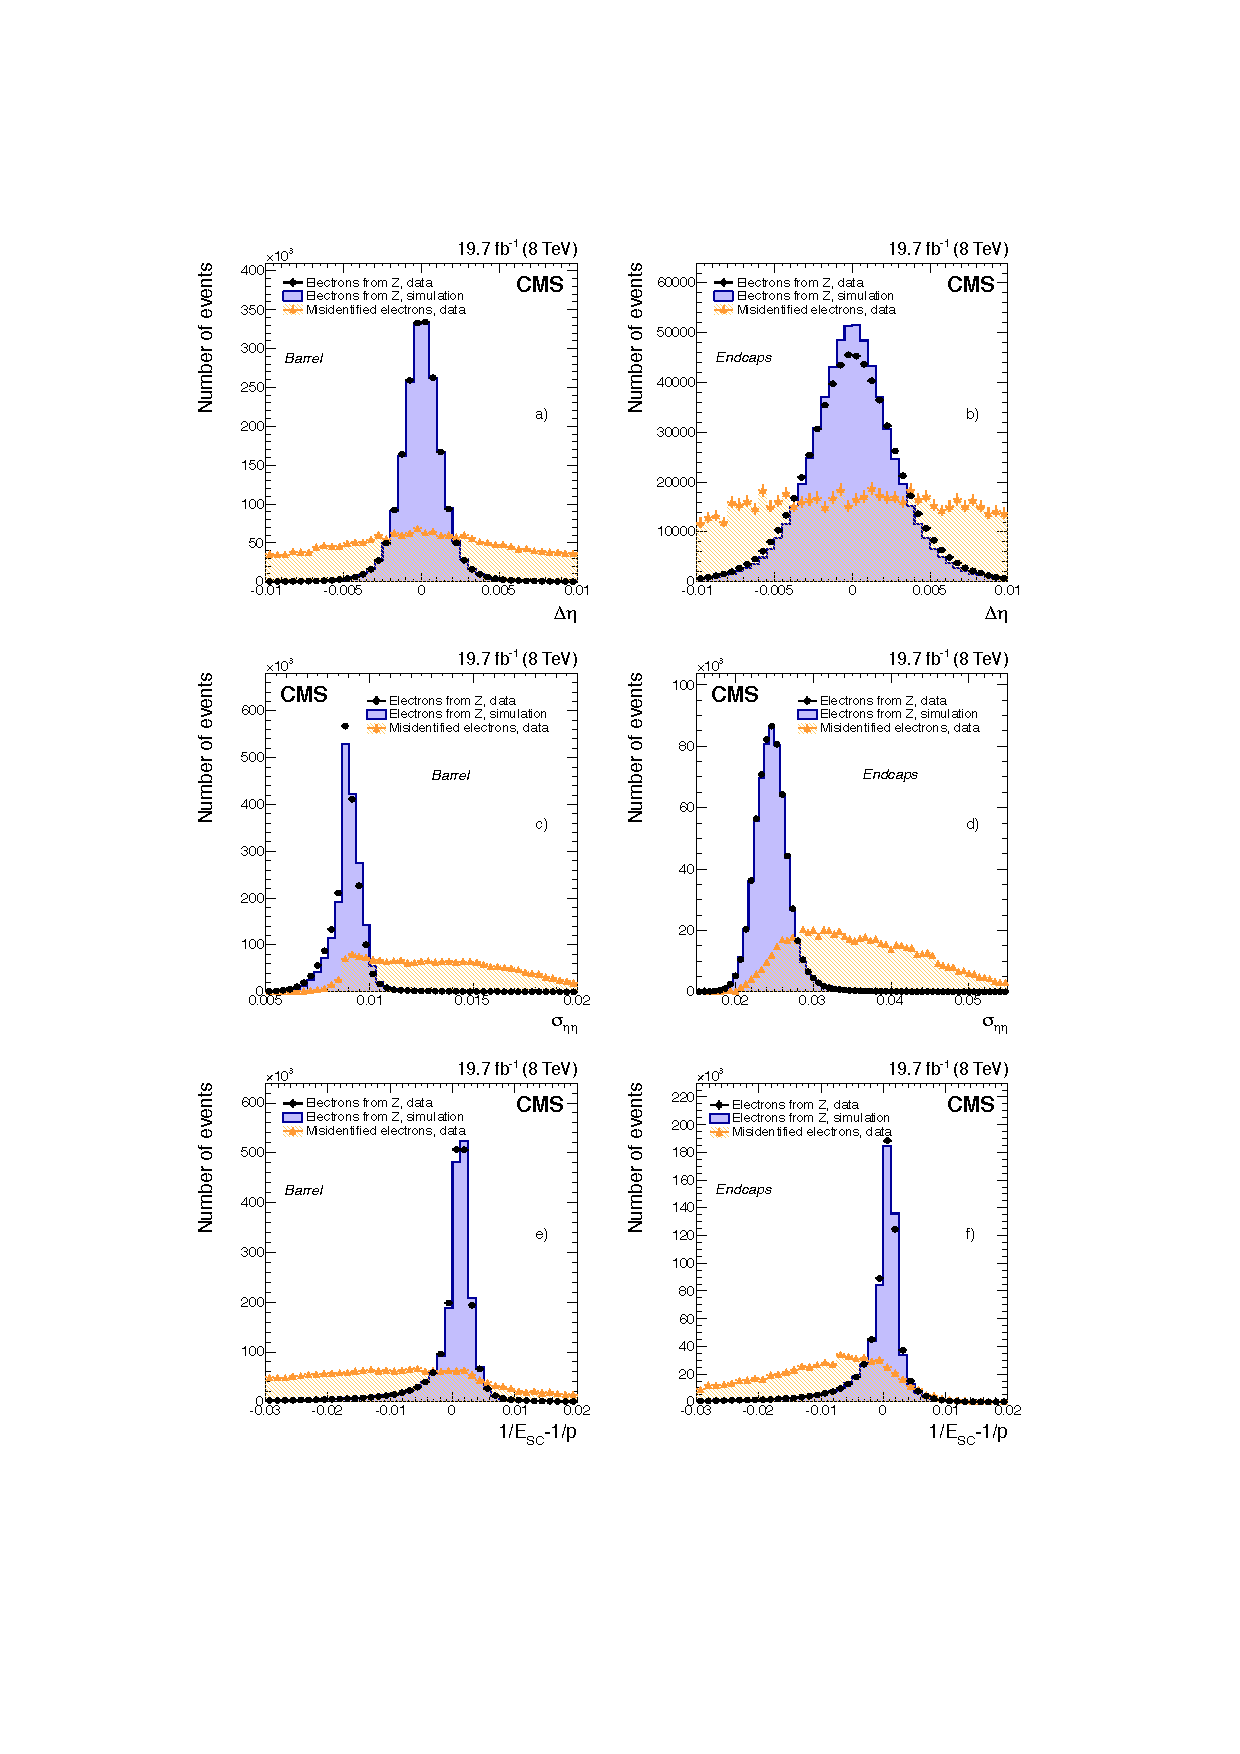
\includegraphics[width=.8\textwidth]{figures/electron_mva_discriminating_distributions.pdf}
      \caption{Some distributions used in the electron MVA that help discriminate between real (prompt) and fake (non-prompt) electrons. Simulation provides a guaranteed way to tag electrons as prompt or not-prompt, and so is used to train the MVA. However, it is important that data and simulation agree in these variables. $\Delta \eta$ and $\sigma_{\eta\eta}$ are variables that characterize the spread of detector hits associated with the electron in the $\eta$ direction. $E_\text{SC}$ is all the energy deposited into the ECAL which is associated to the electron, and $p$ is the electron's momentum. \todo{Do I need to make these plots myself?}}
      \label{fig:electron_mva_discriminating_vars}
    \end{figure}

    The working points for electrons based on the MVA output are shown below:

    \begin{table}[!h]
      \begin{center}
        \caption{\label{tab:elId}  Electron identification working points used in this analysis.}
        \begin{tabular}{rl|rl|l|l}
          \hline
          \multicolumn{2}{c|}{pseudorapidity region} & \multicolumn{2}{c|}{momentum [GeV]} & loose WP & tight WP \\ 
          \hline\hline
          $0<~|\eta|$&$<0.8$     &  10 $<$ ~\pt\ &$<$ 15 &  -0.86 & 0.77 \\ 
          $0<~|\eta|$&$<0.8$     &  15 $<$ ~\pt\ &$<$ 25 &  -0.96+$0.10*\frac{\pt-15}{10}$ & 0.52+$0.25*\frac{\pt-15}{10}$ \\ 
          $0<~|\eta|$&$<0.8$     &   ~\pt\ &$>$ 25       &  -0.96 & 0.52 \\ 
          \hline
          $0.8<~|\eta|$&$<1.479$ &  10 $<$ ~\pt\ &$<$ 15 &  -0.85 & 0.56 \\ 
          $0.8<~|\eta|$&$<1.479$ &  15 $<$ ~\pt\ &$<$ 25 &  -0.96+$0.11*\frac{\pt-15}{10}$ & 0.11+$0.45*\frac{\pt-15}{10}$ \\ 
          $0.8<~|\eta|$&$<1.479$ &   ~\pt\ &$>$ 25       &  -0.96 & 0.11 \\ 
          \hline
          $1.479<~|\eta|$&$<2.5$ &  10 $<$ ~\pt\ &$<$ 15 &  -0.81 & 0.48 \\ 
          $1.479<~|\eta|$&$<2.5$ &  15 $<$ ~\pt\ &$<$ 25 &  -0.95+$0.14*\frac{\pt-15}{10}$ & -0.01+$0.49*\frac{\pt-15}{10}$ \\ 
          $1.479<~|\eta|$&$<2.5$ &  ~\pt\ &$>$ 25        &  -0.95 & -0.01 \\ 
          \hline\hline
        \end{tabular}
        
      \end{center}
    \end{table}

    \clearpage

  \subsection{Muon ID and Isolation} \label{sec:muon_id_and_isolation}

    The muon ID is based purely on a cut-based approach, no MVA is used. Again, the selection criteria is based upon the muon POG, which is documented in more detail at ~\cite{muon_POG}. The selection used for the muon ID and isolation are defined below:

    \begin{table}[!h]
      \begin{center}
        \caption{\label{table:muons} Summary of the muons selection requirements. }
        \begin{tabular}{l|c|c}
          \hline
          \hline
          \multicolumn{3}{c}{Good Muon Requirements} \\
          \hline
          Quantity   &  Tight Requirement & Loose Requirement \\
          \hline
          Quality Muon                      & Must pass   & Must pass     \\
          Fraction of valid tracker hits    & $>$ 0.8     & $>$ 0.8  \\ 
          \hline
          $d_{0}$ (w.r.t. 1st good PV)   & $<0.05$ cm & $<0.05$ cm \\
          $d_{z}$ (w.r.t. 1st good PV)   & $<0.1$ cm  & $<0.1$ cm  \\
          SIP3D                          & $< 8$      & $< 8$      \\
          miniRelIso                     & $<0.20$    & $<0.40$       \\
          \hline
        \end{tabular}
      \end{center}
    \end{table}

    The criteria to be a ``Quality Muon" is given below:
    \begin{table}[!h]
      \begin{center}
        \caption{\label{table:muons} Summary of Quality Muon requirements.}
        \begin{tabular}{l|c}
          \hline
          \hline
          \multicolumn{2}{c}{Quality Muon Requirements} \\
          \hline
          Quantity   &  Requirement \\
          \hline
          Segment compatibility             &$>$ 0.451 \\
          \hline
          \emph{or} & \\
          \hline
          Normalized global-track $\chi^2$  & $<$ 3    \\
          Tracker-Standalone position match & $<$ 12   \\
          Kick finder                       & $<$ 20   \\
          Segment compatibility             & $>$ 0.303 \\
          \hline
          \hline
        \end{tabular}
      \end{center}
    \end{table}

    \todo{brief blurb on global/tracker muons.}

\newpage

  \subsection{Photon Selection} \label{sec:photon_selection}

    Photons are used in this analysis as part of the Z+Hadronic background prediction. The details of this prediction are in \ref{sec:z_+_hadronic}. The bulk of these selections are in order to ensure there is no inefficiency for the trigger for $\gamma +$jets events. 

    \begin{itemize}
      \item \pt $ > 22$ GeV
      \item $|\eta| < 2.4$
      \item No matching pixel track (pixel veto)
      \item There must be a jet candidate of \pt $ >$ 10 GeV matched to the photon within $\DR < 0.3$. 
      The matched jet is required to have a neutral electromagnetic energy fraction of at least 70\%.

      \item We reject photons which have an electron of at least \pt $>$ 10 GeV within $\DR < 0.2$
      in order to reject conversions from electrons from W decays which are accompanied by real \MET.

      \item We reject photons which are aligned with the \MET to within 0.4 radians in phi.
      \item To ensure full efficiency with respect to the isolated photon triggers used, we apply the following additional cuts:
      \begin{itemize}
        \item ratio of the energy of the energy of the photon's 3X3 supercluster to the photons 5X5 supercluster (R9) $>$ 0.92
        \item $\frac{H}{E} < 0.2$ %\fixme{is this the HLT H/E or still offline?}
        \item hollow track isolation $<$ 3 GeV
        \item photons with $|\eta| < 1.4$ have ECAL pfcluster iso $<$ 3 GeV + \pt ($\gamma$) * 0.0053
        \item photons with $|\eta| < 1.4$ have HCAL pfcluster iso $<$ 7 GeV + \pt ($\gamma$) * 0.014
        \item photons with $|\eta| > 1.6$ have ECAL pfcluster iso $<$ 3 GeV + \pt ($\gamma$) * 0.0034
        \item photons with $|\eta| > 1.6$ have HCAL pfcluster iso $<$ 7 GeV + \pt ($\gamma$) * 0.0139
      \end{itemize}
    \end{itemize}

  \subsection{Jet Selection} \label{sec:jet_selection}

  Jets are selected from the particle flow selection and are refined via ``charged hadron subtraction" and ``jet energy corrections" described in \ref{sec:jets}. In this analysis, we distinguish between jets and ``b-tagged jets." B-tagging is described in \ref{sec:b-tagging}, but it comes down to a numerical quantity assigned to each jet called its \emph{b-tag csv value}. If the csv value is large enough, a jet is considered likely to have been generated by a free bottom quark. 

      \begin{table}[!h]
      \begin{center}
        \caption{\label{table:muons} Summary Of Good Jet Requirements.}
        \begin{tabular}{l|c|c}
          \hline
          \hline
          \multicolumn{3}{c}{Jet Selections} \\
          \hline
          \hline
          Quantity                  & \multicolumn{2}{c}{ Cut Value } \\
          \hline
          $\abs{\eta}$              & \multicolumn{2}{c}{$< 2.4$}   \\
          Lepton Veto               & \multicolumn{2}{c}{Not within $\abs{\DR} < 0.4$ of a tight lepton} \\
          Photon Veto               & \multicolumn{2}{c}{Not within $\abs{\DR} < 0.4$ of a good photon } \\
          Neutral Hadron Fraction   & \multicolumn{2}{c}{ $< 0.99$} \\
          Neutral EM fraction       & \multicolumn{2}{c}{ $< 0.99$} \\
          Charged hadron fraction   & \multicolumn{2}{c}{ $> 0   $} \\
          Charged multiplicity      & \multicolumn{2}{c}{ $> 0   $} \\
          Charged EM fraction       & \multicolumn{2}{c}{ $< .99 $} \\
          Number of constituents    & \multicolumn{2}{c}{ $> 1   $} \\
          \hline
          \hline
          Quantity                  &  Jet Requirement & B-tagged Jet Requirement\\
          \hline
          \pt                       & $> 35\; \GeV $     & $> 25\; \GeV$   \\
          B-tag CSV                 & None             & $> 0.8484$    \\
          \hline
          \hline
        \end{tabular}
      \end{center}
    \end{table}

  \subsection{Isolated Tracks} \label{sec:isolated_tracks}
  In addition to vetoing events which have extra loose leptons, a typically more inclusive veto is applied to kill events which might have an extra prompt lepton based on the identification of an isolated charged object. 

  To distinguish these types of objects, we introduce the notion of ``track isolation," defined as the total energy of all the particle flow charged candidates that trace back to within $\abs{dz} < 0.1$ cm of the primary vertex within a cone of $\abs{\DR} <0.3$ about the lepton.\footnote{Notice that the miniRelIso we defined above was defined as a relative isolation, the energy in a cone divided by the \pt of the object in question, track isolation as defined here has units of energy.}

  There are two types of isolated tracks, those that are seeded by particle flow charged hadron candidates, and those that are seeded by particle flow electron or muon candidates. The criteria on top of the particle flow identification for these two sources are listed in the tables below:

  \begin{table}[!h]
      \begin{center}
        \caption{\label{table:muons} Summary Of Isolated Track Requirements.}
        \begin{tabular}{l|c|c}
          \hline
          \hline
          \multicolumn{3}{c}{Isolated Track Selections} \\
          \hline
          \hline
          Quantity                  &  Charged Hadronic Requirement & Light Lepton Requirement\\
          \hline
          \pt                       & $> 10\; \GeV $                & $> 5\; \GeV$           \\
          Vertex Association\footnote{PVTight means the particle was closer to the primary vertex than any other reconstructed vertex. PVUsedInFit means the particle was used to define the primary vertex. There are more details in the glossary.}     & PVTight or PVUsedInFit  & PVTight or PVUsedInFit \\ 
          Track Isolation           & $<8\; \GeV$                   & $<8\; \GeV$             \\
          Track Isolation / \pt     & $<0.2$                        & $<0.1$                  \\
          $\abs{dz}$                & $< 0.1$ cm                    & $< 0.1$ cm              \\
          \hline
          \hline
        \end{tabular}
      \end{center}
    \end{table}

\section{Event Selection}

  The selection of events can be broken into several stages. Though each of these regions will be expanded upon in the following sections, in broad strokes there 4 separate final states used to accomplish this analysis. These final states define the signal regions and 3 control regions used to conduct this search:

  \begin{description}
    \bitem{Search Regions (SR)} Events with two opposite charge and same flavor light leptons build our search regions, we have either a $e^+e^-$ or a $\mu^+ \mu^-$ pair in each event.
    \bitem{Flavor Symmetric Control Regions (FSCR)} Events with two opposite charge and different flavor light leptons build our flavor symmetric control region, we have either a $e^+\mu^-$ or a $\mu^+ e^-$ pair in each event. This region is used to predict the flavor symmetric background.
    \bitem{\MET Templates Control Region (MTCR)} Events with a single photon are used to construct the \MET templates control region. 
    \bitem{EWK Contamination Closure Region (ECCR)} Events with a photon and muon are used to check the modeling of the ``EWK contamination" in the \MET Templates prediction, described in section \ref{sec:ewk_subtraction}.
  \end{description}

  The CMS datasets which seed these events are described in \ref{sec:datasets}.
  
  \subsection{Lepton Selection}
    The following are the requirements for events with two light leptons, i.e. for the search regions and for the FSCR. The requirements for the MTCR and ECCR are described in section \ref{sec:met_templates_control_region} and \ref{sec:ewk_subtraction_closure_region} respectively. 

    Light lepton candidates are tagged by the particle flow algorithm described in section \ref{sec:particle_flow}. In addition to the list below, leptons must also pass preselection ID and isolation requirements which differ depending on their flavor, but are described in \ref{sec:electron_id_and_isolation} and \ref{sec:muon_id_and_isolation} above.

    \begin{itemize}
      \item The (sub)leading lepton in each event must have at least (20) 25 GeV of transverse momentum. These points were selected so that the event would be in the "trigger turn-on" described in \ref{sec:event_triggering}.
      \item The pseudorapidity for each lepton must be within the inner tracker's fiducial area, namely $\left|\eta\right| < 2.4$
      \item No lepton should be in the ``dead zone" described in section \ref{sec:fiducial_area}, this is in the range $1.4 < \left|\eta\right| < 1.6$
      \item For the search region, events must have exactly one pair of opposite charge same flavor (OCSF) light leptons, for the FSCR events must have exactly one pair of opposite charge and different flavor (OCDF) light leptons.
      \item The mass constructed out of the sum of lepton vectors (dilepton mass) must be between 86 and 96 GeV.
      \item The transverse momentum of the dilepton system must be at least 25 GeV in order to ensure the Z+hadronic background prediction has enough statistics. This is explained in more detail in \ref{sec:z_+_hadronic}.
    \end{itemize}

  \subsection{Event Vetos}
    Events are generally vetoed across all search, control, and closure regions if any of the following are true:

    \begin{description}
      \bitem{Isolated Track Veto} Events with an isolated track, defined in \ref{sec:isolated_tracks}.
      \bitem{\MET Filters} Events where any of the ``\MET Filters", described in section \ref{sec:met_filters}, are true.
    \end{description}

    Dilepton events specifically, those within the SRs and FSCRs, are vetoed under the following conditions:

      \begin{description}
        \bitem{Lepton Cone Isolation} The two tight leptons are within a cone of $\Delta R < 0.1$ of each other.
        \bitem{Extra Lepton Veto} There is an additional loose or tighter lepton in the event. In other words, event with three or more loose IDed leptons are vetoed. IDs are defined in \ref{sec:electron_id_and_isolation} and \ref{sec:muon_id_and_isolation}. 
      \end{description}

  \subsection{Search Regions}
    Electroweak search regions and strong search regions

  \subsection{Flavor Symmetric Control Region} \label{sec:flavor_symmetric_control_region}
    A flavor symmetric control region in constructed for every search region by flipping the requirement for an OCSF dilepton pair to a OCDF dilepton pair. The number of events in these regions is used to predict the background of events where the two leptons come from a pair of W bosons as described in \ref{sec:flavor_symmetric_background}

  \subsection{\MET Templates Closure Region} \label{sec:met_templates_control_region}

  \subsection{EWK Subtraction Closure Region} \label{sec:ewk_subtraction_closure_region}



\section{Background Estimation Methods} \label{sec:background_estimation_methods}
  Fakes are taken care of by the flavor symmetric BG.

  For the signal regions, we select events with opposite charge and same flavor dilepton pairs, for the flavor-symmetric background prediction, we select events with same sign and same flavor dilepton pairs, for the \MET templates prediction, we select from single photon events which are seeded by an entirely different dataset.

  \subsection{Z + Hadronic} \label{sec:z_+_hadronic}
  \pt of the Z greater than 25 GeV for photon trigger.
    
    \subsubsection{Contamination From Events With Real \MET (Electroweak Subtraction)} \label{sec:ewk_subtraction}
      Explain the EWK subtraction method here.

    \subsubsection{Electroweak Subtraction Control Region} \ref{sec:ewk_subtraction_control_region}

  \subsection{Flavor Symmetric Background} \label{sec:flavor_symmetric_background}

  \subsection{Z + $\nu$} \label{sec:z_+_neutrino}

\section{Results} \label{sec:results}
  \subsection{Strong Search Regions} \label{sec:strong_search_regions}
    In this section, we show the search results for the strong signal regions. Figure \ref{fig:results_SR_str} shows the results visually, each search region is shown binned in \MET, the background predictions are broken down as described in \ref{sec:background_estimation_methods} and uncertainty bands are shown as a hashing that captures all sources described above. The number of events in data seen are shown as black dots in the figures. The same data is shown numerically in table \ref{tab:results_SR_str}.

    \begin{table}[!h]
      \scriptsize
      \centering
      \caption{\label{tab:results_SR_str} \todo{identical cap to AN}
      Results are shown for the strong signal regions.
      The uncertainties shown include both statistical and systematic errors. Note that the 50-100 \MET bin agrees perfectly by construction as it is used to normalize the DY prediction. See figure~\ref{fig:results_SR_str}~for the corresponding plots.
      }
      \begin{center}
        \begin{tabular} {l | l | l | l | l | l }
          SRA & \MET [GeV]  & 50-100 & 100-150 & 150-250 & 250+ \\ \hline 
          & Template  & 208.5$\pm$16.1 & 13.6$\pm$3.1 & 2.5$\pm$0.9 & 3.3$\pm$2.4 \\
          & FS  & $0.4^{+0.3}_{-0.2}$  & $0.4^{+0.3}_{-0.2}$  & $0.2^{+0.2}_{-0.1}$  & $0.2^{+0.2}_{-0.1}$  \\
          & Rares  & 1.1$\pm$0.4 & 0.8$\pm$0.3 & 1.4$\pm$0.4 & 2.4$\pm$0.8 \\ 
          & Sum  & $210.0^{+16.1}_{-16.1}$  & $14.8^{+3.2}_{-3.2}$  & $4.0^{+1.0}_{-1.0}$  & $5.9^{+2.5}_{-2.5}$ \\ 
          & Data  & 210 & 23 & 5 & 4 \\ \hline 


          SRAb & \MET [GeV]  & 50-100 & 100-150 & 150-250 & 250+ \\ \hline 
          & Template  & 92.2$\pm$10.4 & 8.2$\pm$2.1 & 1.2$\pm$0.5 & 0.5$\pm$0.3 \\
          & FS  & $1.9^{+0.7}_{-0.7}$  & $2.3^{+0.8}_{-0.8}$  & $1.7^{+0.7}_{-0.6}$  & $0.1^{+0.2}_{-0.1}$  \\
          & Rares  & 1.9$\pm$0.4 & 1.9$\pm$0.4 & 2.0$\pm$0.5 & 1.8$\pm$0.6 \\ 
          & Sum  & $96.0^{+10.4}_{-10.4}$  & $12.4^{+2.3}_{-2.3}$  & $4.9^{+1.0}_{-1.0}$  & $2.5^{+0.7}_{-0.7}$ \\ 
          & Data  & 96 & 14 & 7 & 1 \\ \hline 


          SRB & \MET [GeV]  & 50-100 & 100-150 & 150-250 & 250+ \\ \hline 
          & Template  & 130.1$\pm$12.8 & 12.8$\pm$2.3 & 0.9$\pm$0.3 & 0.4$\pm$0.2 \\
          & FS  & $0.3^{+0.2}_{-0.2}$  & $0.4^{+0.3}_{-0.2}$  & $0.4^{+0.3}_{-0.2}$  & $0.1^{+0.2}_{-0.1}$  \\
          & Rares  & 0.6$\pm$0.2 & 0.3$\pm$0.1 & 0.7$\pm$0.2 & 1.2$\pm$0.4 \\ 
          & Sum  & $131.0^{+12.8}_{-12.8}$  & $13.6^{+2.4}_{-2.4}$  & $2.0^{+0.5}_{-0.5}$  & $1.6^{+0.5}_{-0.4}$ \\ 
          & Data  & 131 & 10 & 4 & 0 \\ \hline 


          SRBb & \MET [GeV]  & 50-100 & 100-150 & 150-250 & 250+ \\ \hline 
          & Template  & 37.9$\pm$6.7 & 7.7$\pm$3.1 & 4.0$\pm$3.3 & 0.1$\pm$0.1 \\
          & FS  & $0.7^{+0.4}_{-0.3}$  & $1.4^{+0.6}_{-0.5}$  & $1.1^{+0.5}_{-0.4}$  & $0.2^{+0.2}_{-0.1}$  \\
          & Rares  & 1.3$\pm$0.4 & 2.0$\pm$0.5 & 2.3$\pm$0.6 & 1.0$\pm$0.3 \\ 
          & Sum  & $40.0^{+6.8}_{-6.8}$  & $11.1^{+3.2}_{-3.2}$  & $7.4^{+3.4}_{-3.4}$  & $1.3^{+0.4}_{-0.3}$ \\ 
          & Data  & 40 & 10 & 5 & 0 \\ \hline 


          SRC & \MET [GeV]  &  50-100 &  100-150 & \multicolumn{2}{l}{ 150+ } \\ \hline 
          & Template  &  23.8$\pm$5.5 &  1.2$\pm$0.4 & \multicolumn{2}{l}{ 0.1$\pm$0.1 } \\ 
          & FS  &  $0.1^{+0.2}_{-0.1}$  &  $0.4^{+0.3}_{-0.2}$  & \multicolumn{2}{l}{ $0.1^{+0.2}_{-0.1}$  } \\ 
          & Rares  &  0.2$\pm$0.1 &  0.1$\pm$0.1 & \multicolumn{2}{l}{ 0.5$\pm$0.2 } \\ 
          & Sum  &  $24.0^{+5.5}_{-5.5}$  &  $1.7^{+0.5}_{-0.5}$  & \multicolumn{2}{l}{ $0.7^{+0.3}_{-0.2}$ } \\ 
          & Data  &  24 &  4 & \multicolumn{2}{l}{ 0 } \\ \hline 


          SRCb & \MET [GeV]  &  50-100 &  100-150 & \multicolumn{2}{l}{ 150+ } \\ \hline 
          & Template  &  9.9$\pm$3.7 &  0.1$\pm$0.5 & \multicolumn{2}{l}{ 0.0$\pm$0.3 } \\ 
          & FS  &  $0.1^{+0.2}_{-0.1}$  &  $0.0^{+0.1}_{-0.0}$  & \multicolumn{2}{l}{ $0.3^{+0.2}_{-0.2}$  } \\ 
          & Rares  &  0.0$\pm$0.1 &  0.6$\pm$0.2 & \multicolumn{2}{l}{ 0.6$\pm$0.2 } \\ 
          & Sum  &  $10.0^{+3.7}_{-3.7}$  &  $0.8^{+0.5}_{-0.5}$  & \multicolumn{2}{l}{ $0.9^{+0.5}_{-0.4}$ } \\ 
          & Data  &  10 &  2 & \multicolumn{2}{l}{ 2 } \\ \hline 

        \end{tabular}
      \end{center}
    \end{table}

    \begin{figure}[!htb]
      \centering
      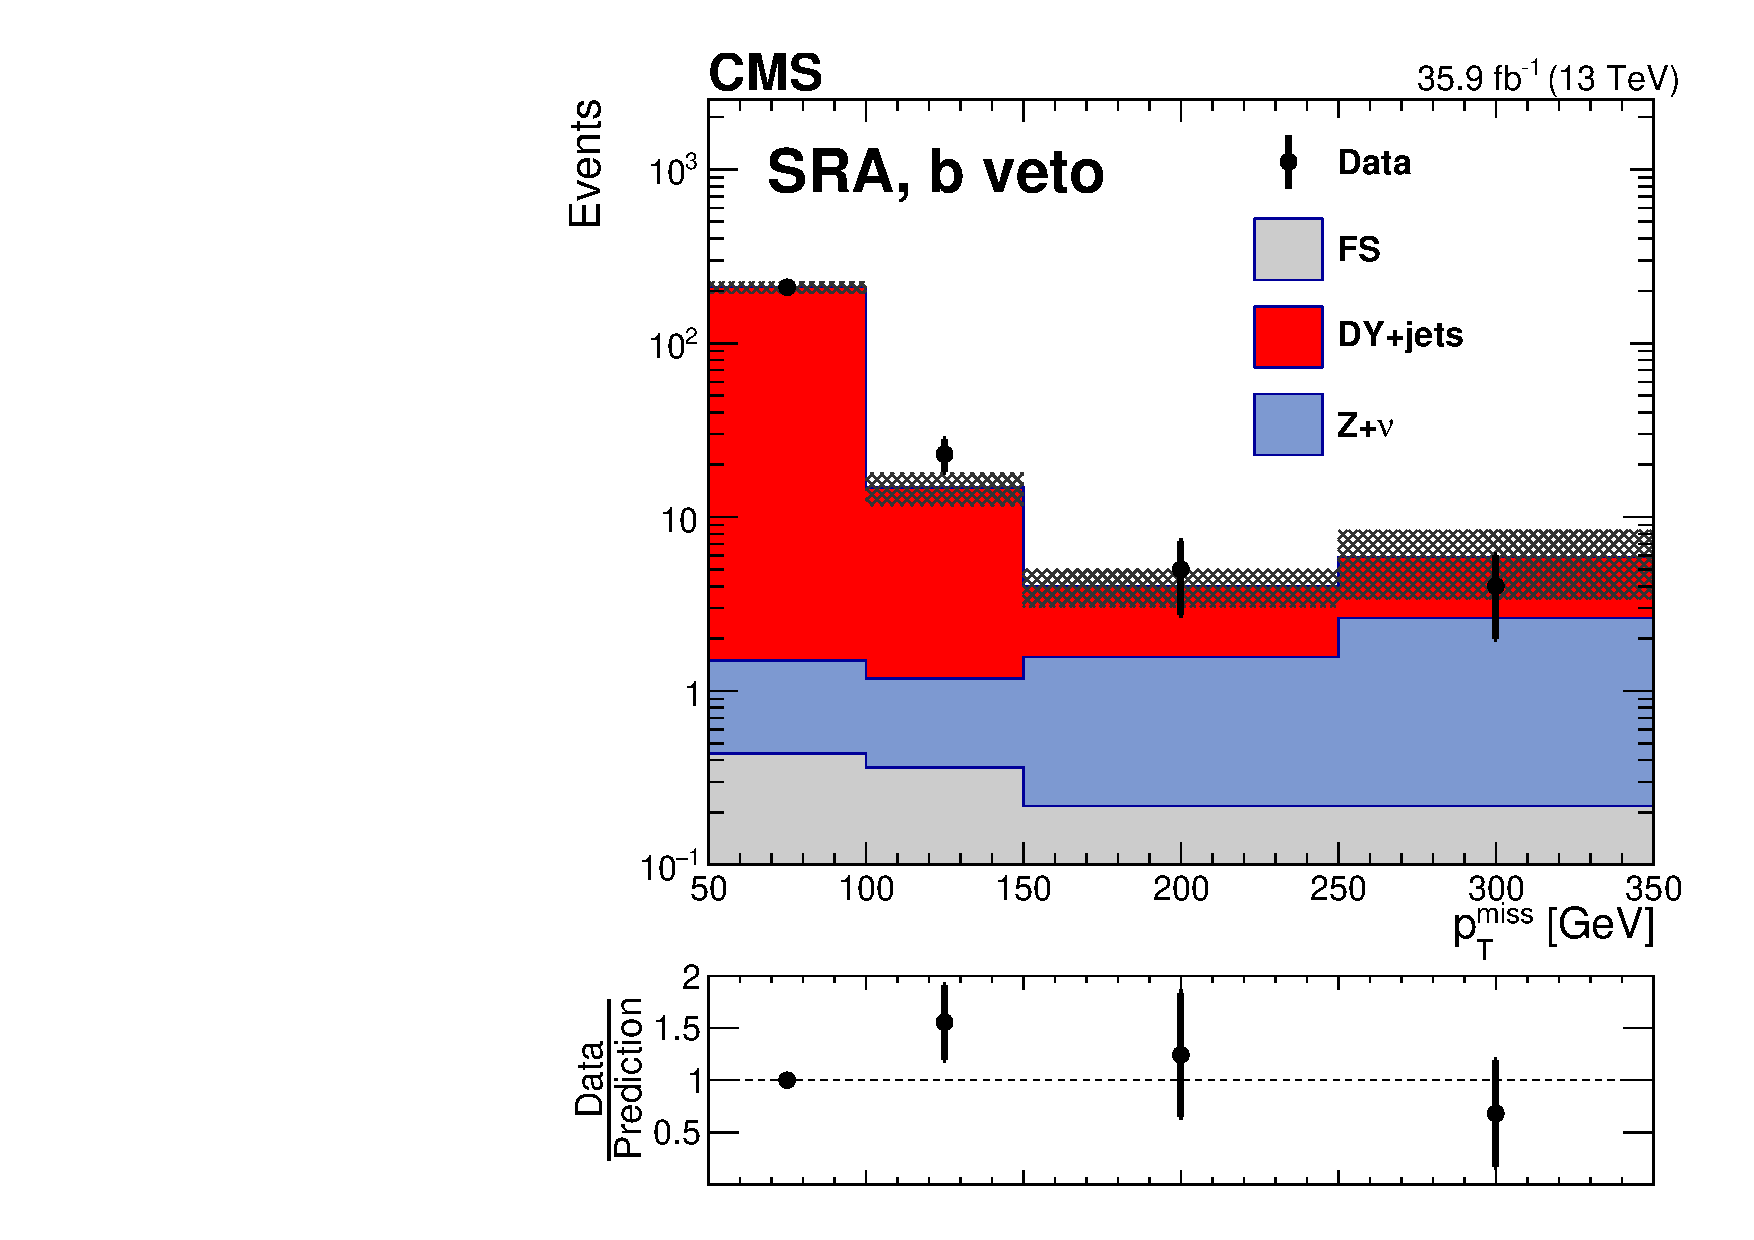
\includegraphics[width=0.35\linewidth]{figures/results/h_met_SR_2jbv.pdf}%
      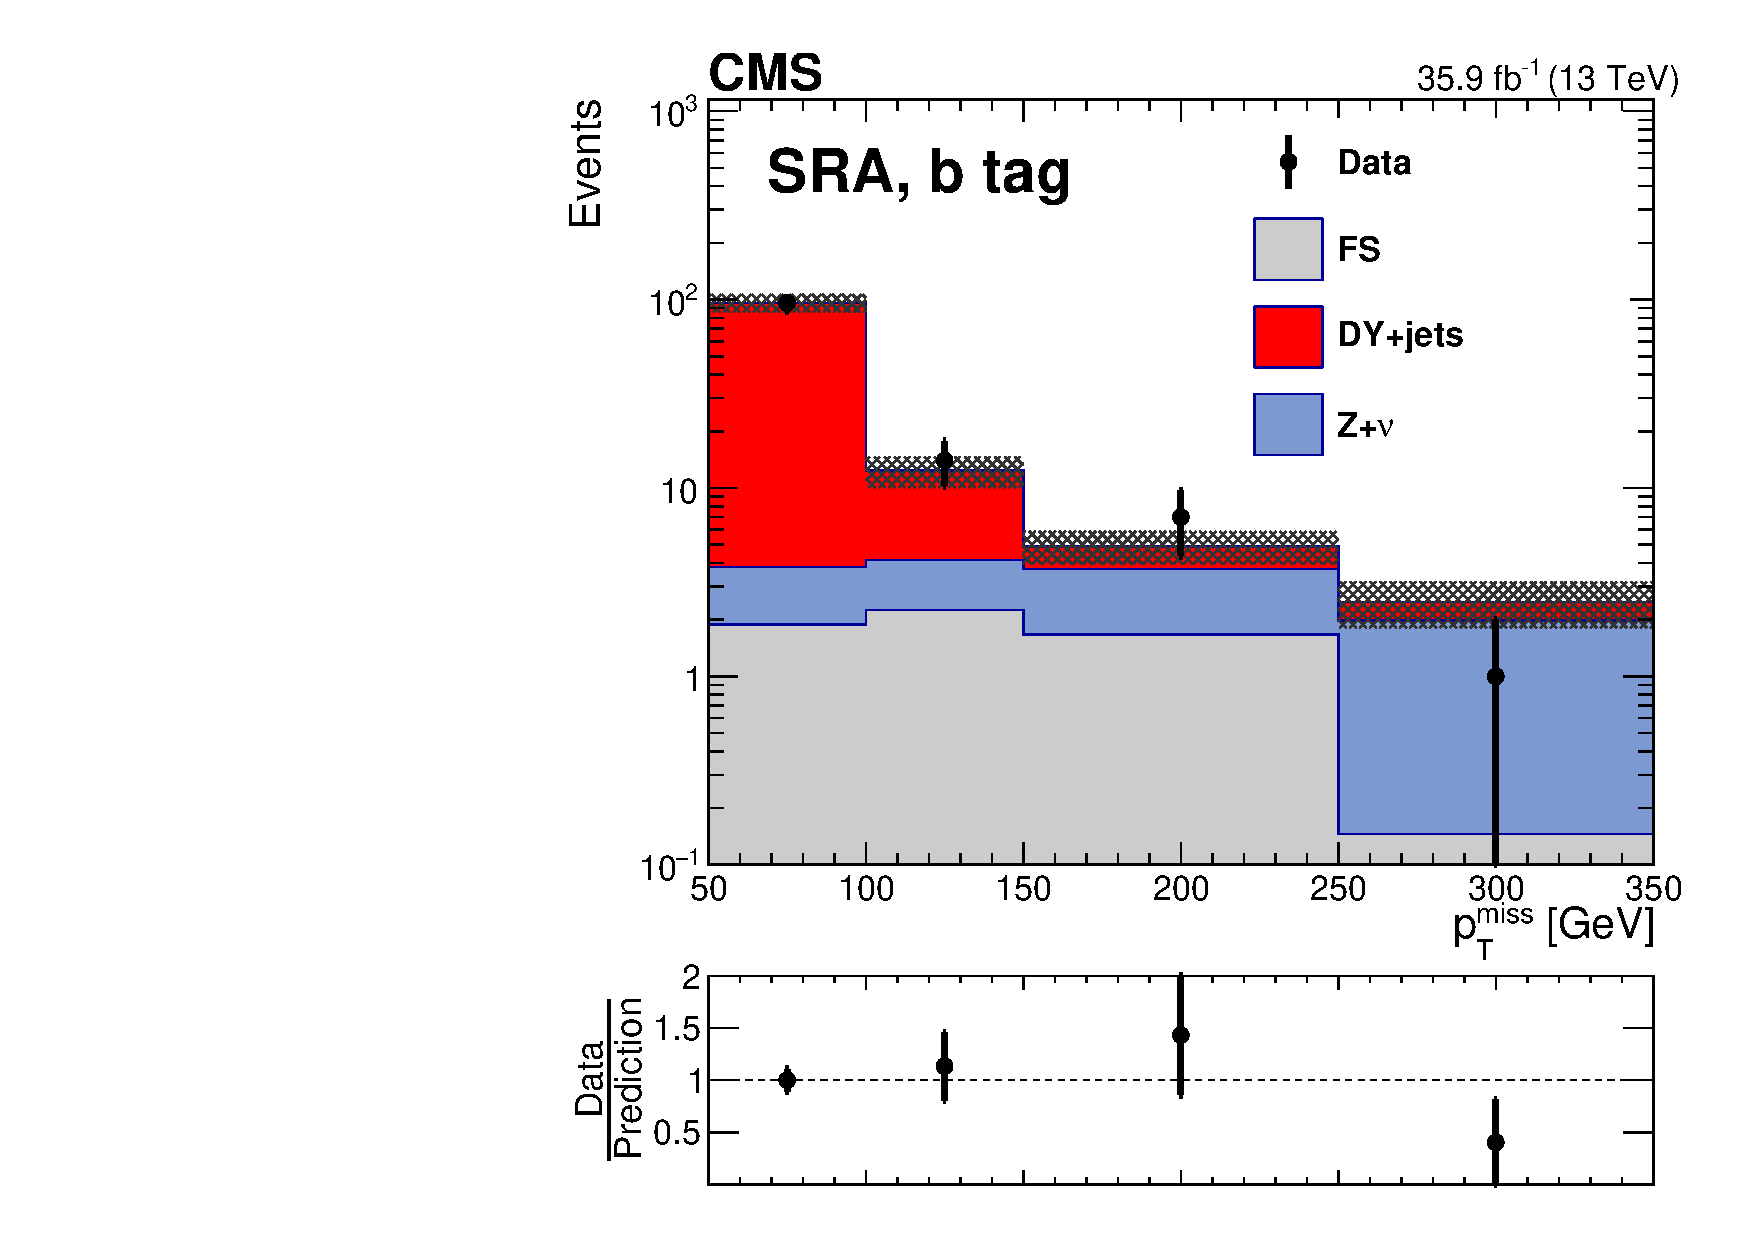
\includegraphics[width=0.35\linewidth]{figures/results/h_met_SR_2jbt.pdf}
      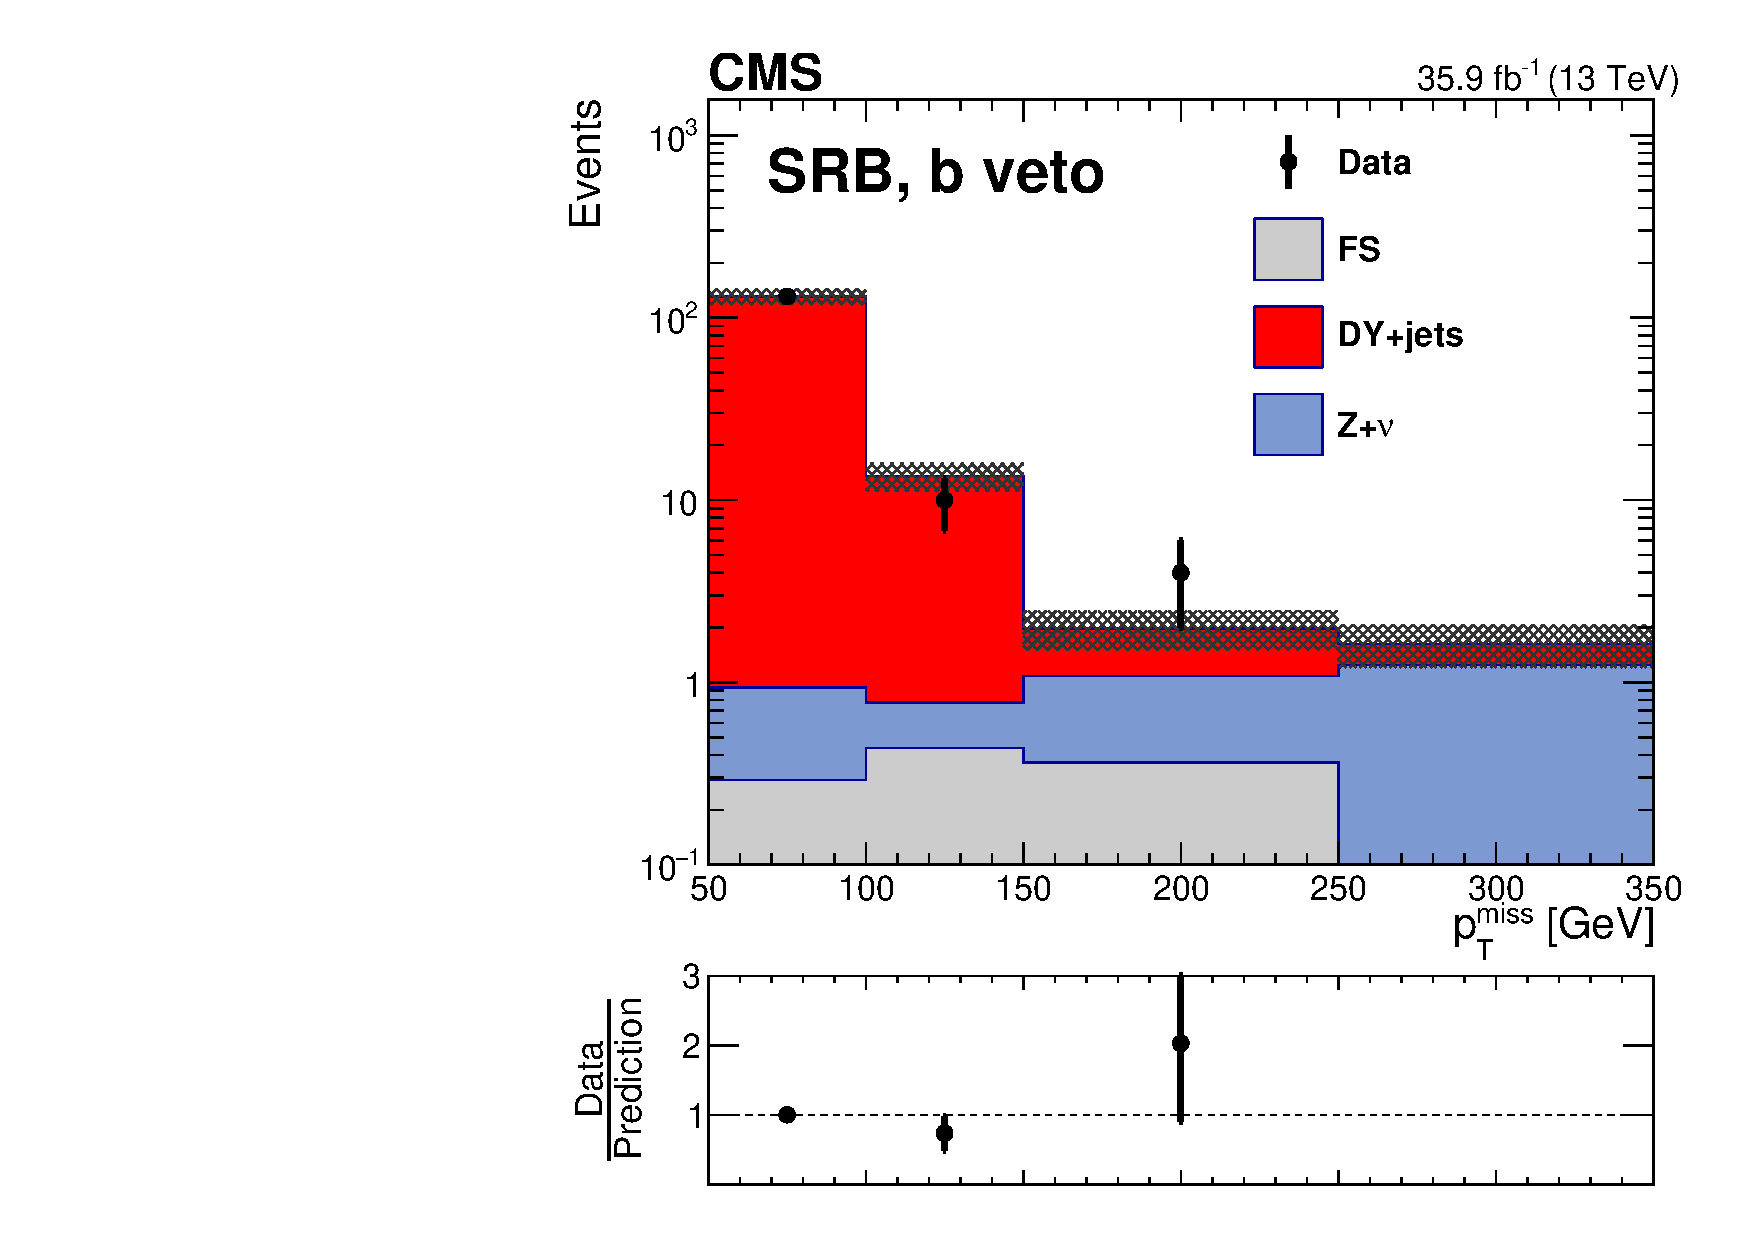
\includegraphics[width=0.35\linewidth]{figures/results/h_met_SR_4jbv.pdf}%
      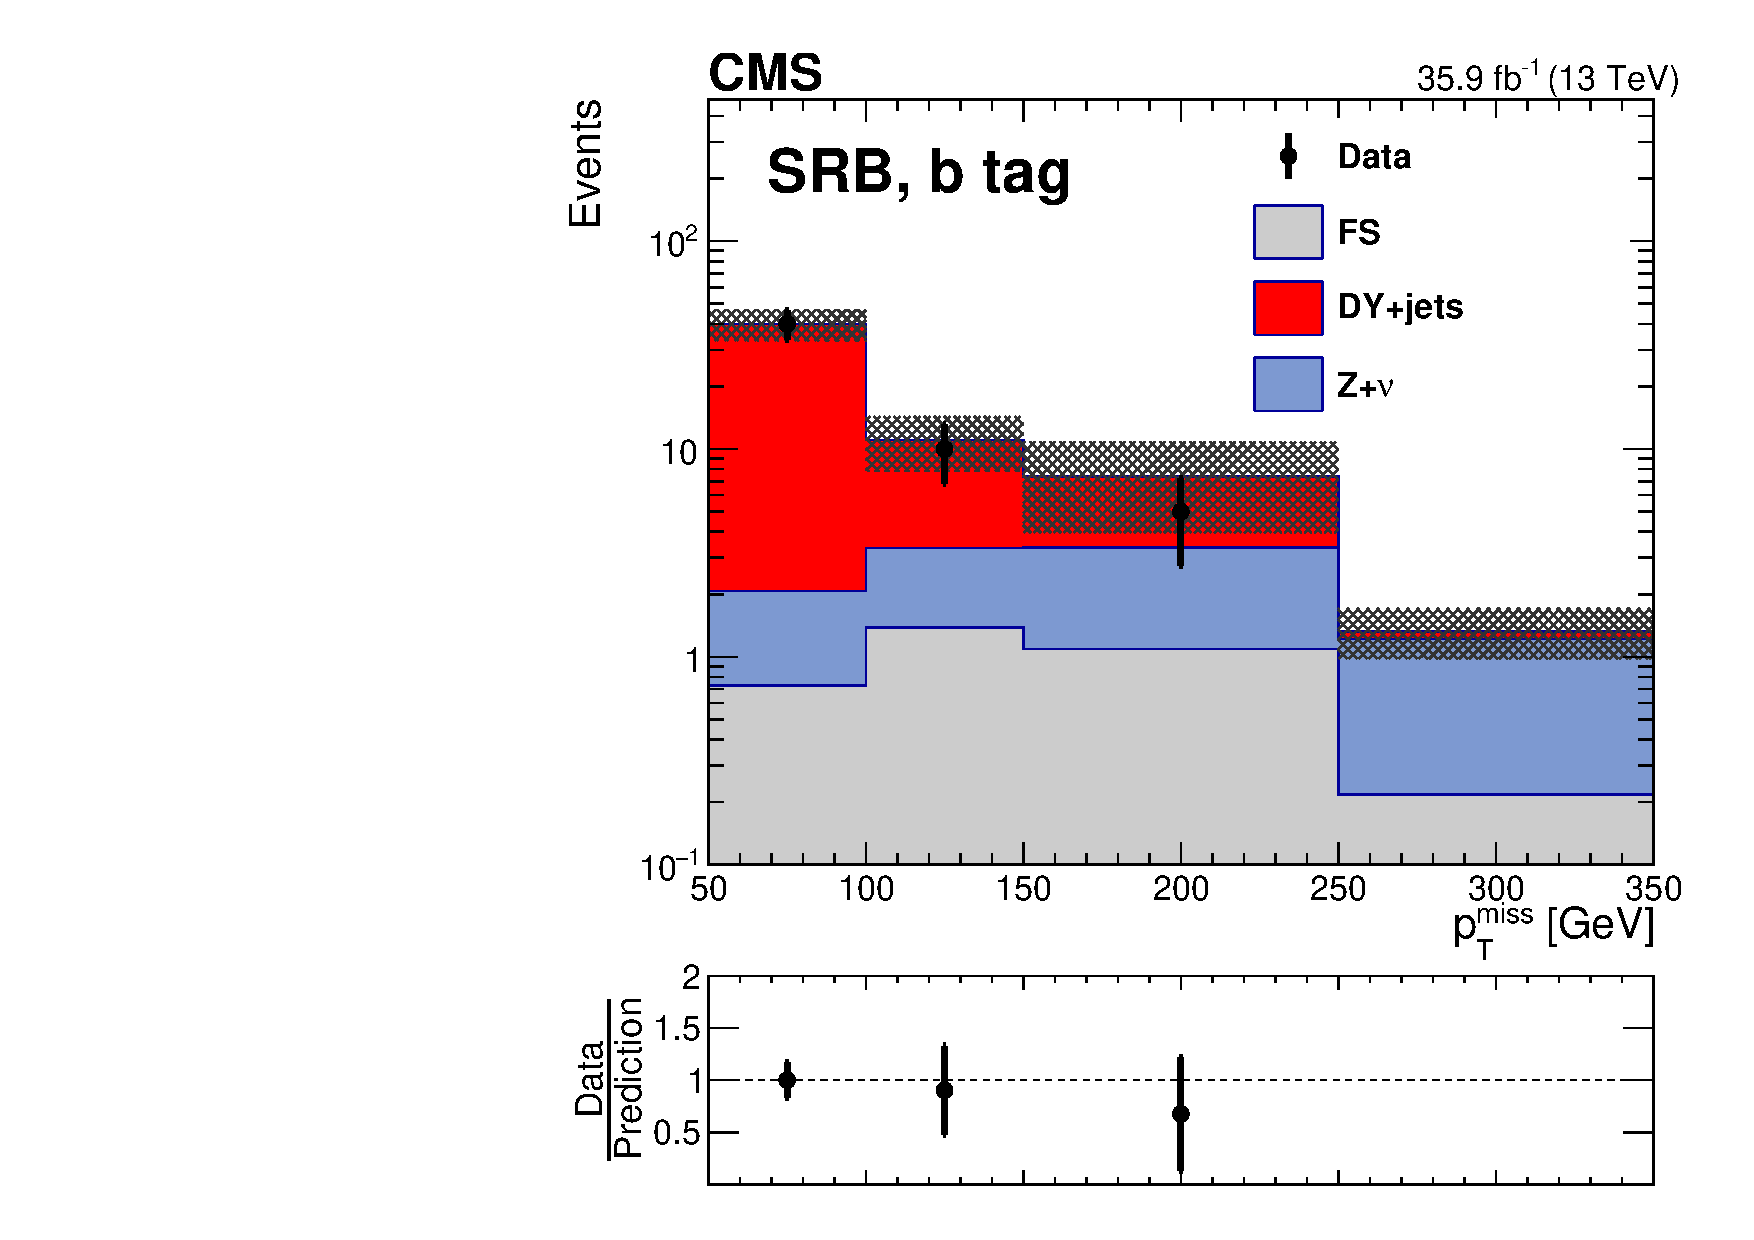
\includegraphics[width=0.35\linewidth]{figures/results/h_met_SR_4jbt.pdf}
      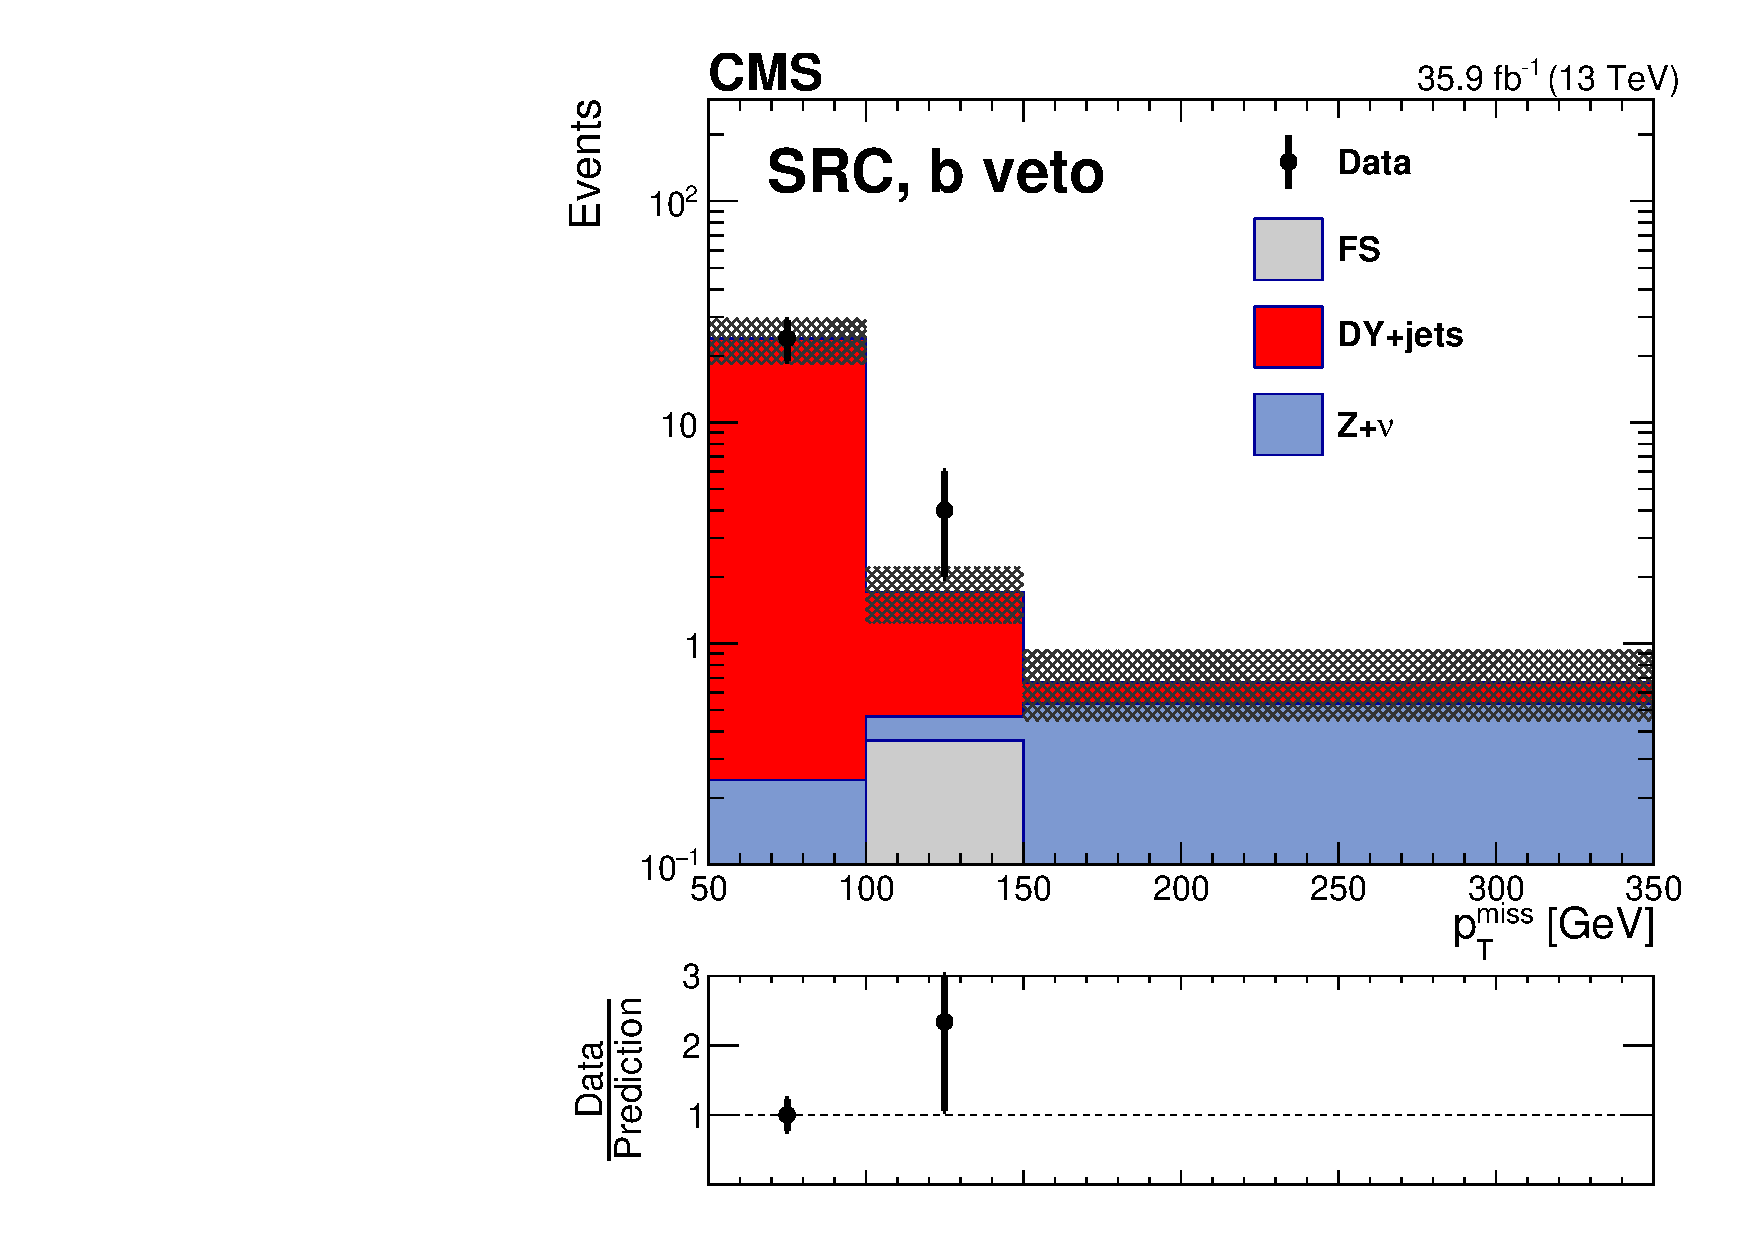
\includegraphics[width=0.35\linewidth]{figures/results/h_met_SR_6jbv.pdf}%
      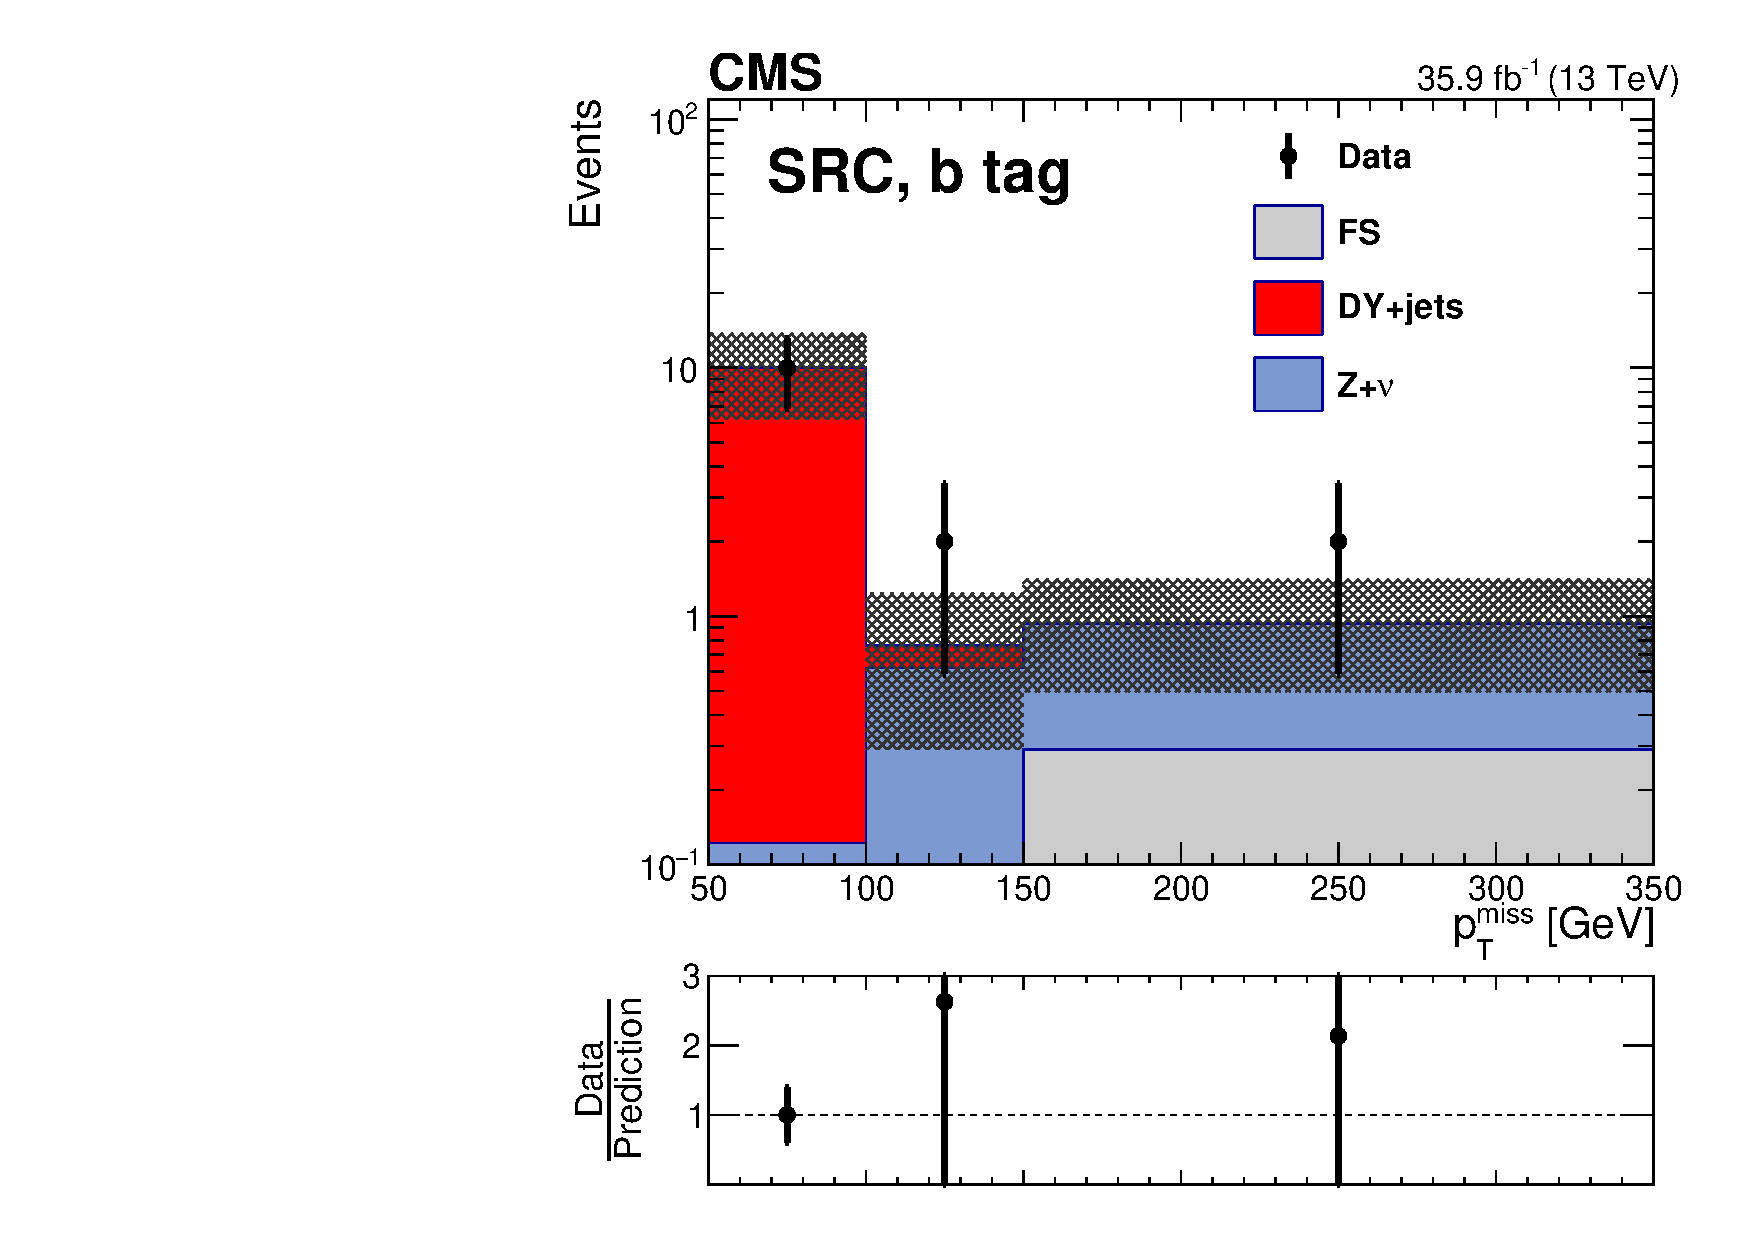
\includegraphics[width=0.35\linewidth]{figures/results/h_met_SR_6jbt.pdf}
      \caption{\label{fig:results_SR_str} \todo{identical cap to AN}
      The \MET distribution is shown for data vs. the data-driven predictions in the strong signal regions with $\nb = 0$ (left) and $\nb \geq 1$ (right).
      The top row shows events in SRA which are required to have 2-3 jets and \HT\ $>$ 500 (200)~GeV for events with exactly 0 bjets (at least one bjet),
      the second row shows events in SRB which are required to have 4-5 jets and \HT\ $>$ 500 (200)~GeV for events with exactly 0 bjets (at least one bjet),
      and the bottom row shows events in SRC which are required to have $\geq$~6 jets.
      Note that the 50-100 \MET bin agrees perfectly by construction as it is used to normalize the DY prediction. The yields for these plots are shown in table~\ref{tab:results_SR_str}.
      }
    \end{figure}

  \clearpage

  \subsection{Electroweak Search Regions}

    The following shows the results for the electroweak search regions. 

    \begin{figure}[!h]
      \centering
      \begin{tabular}{cc}
        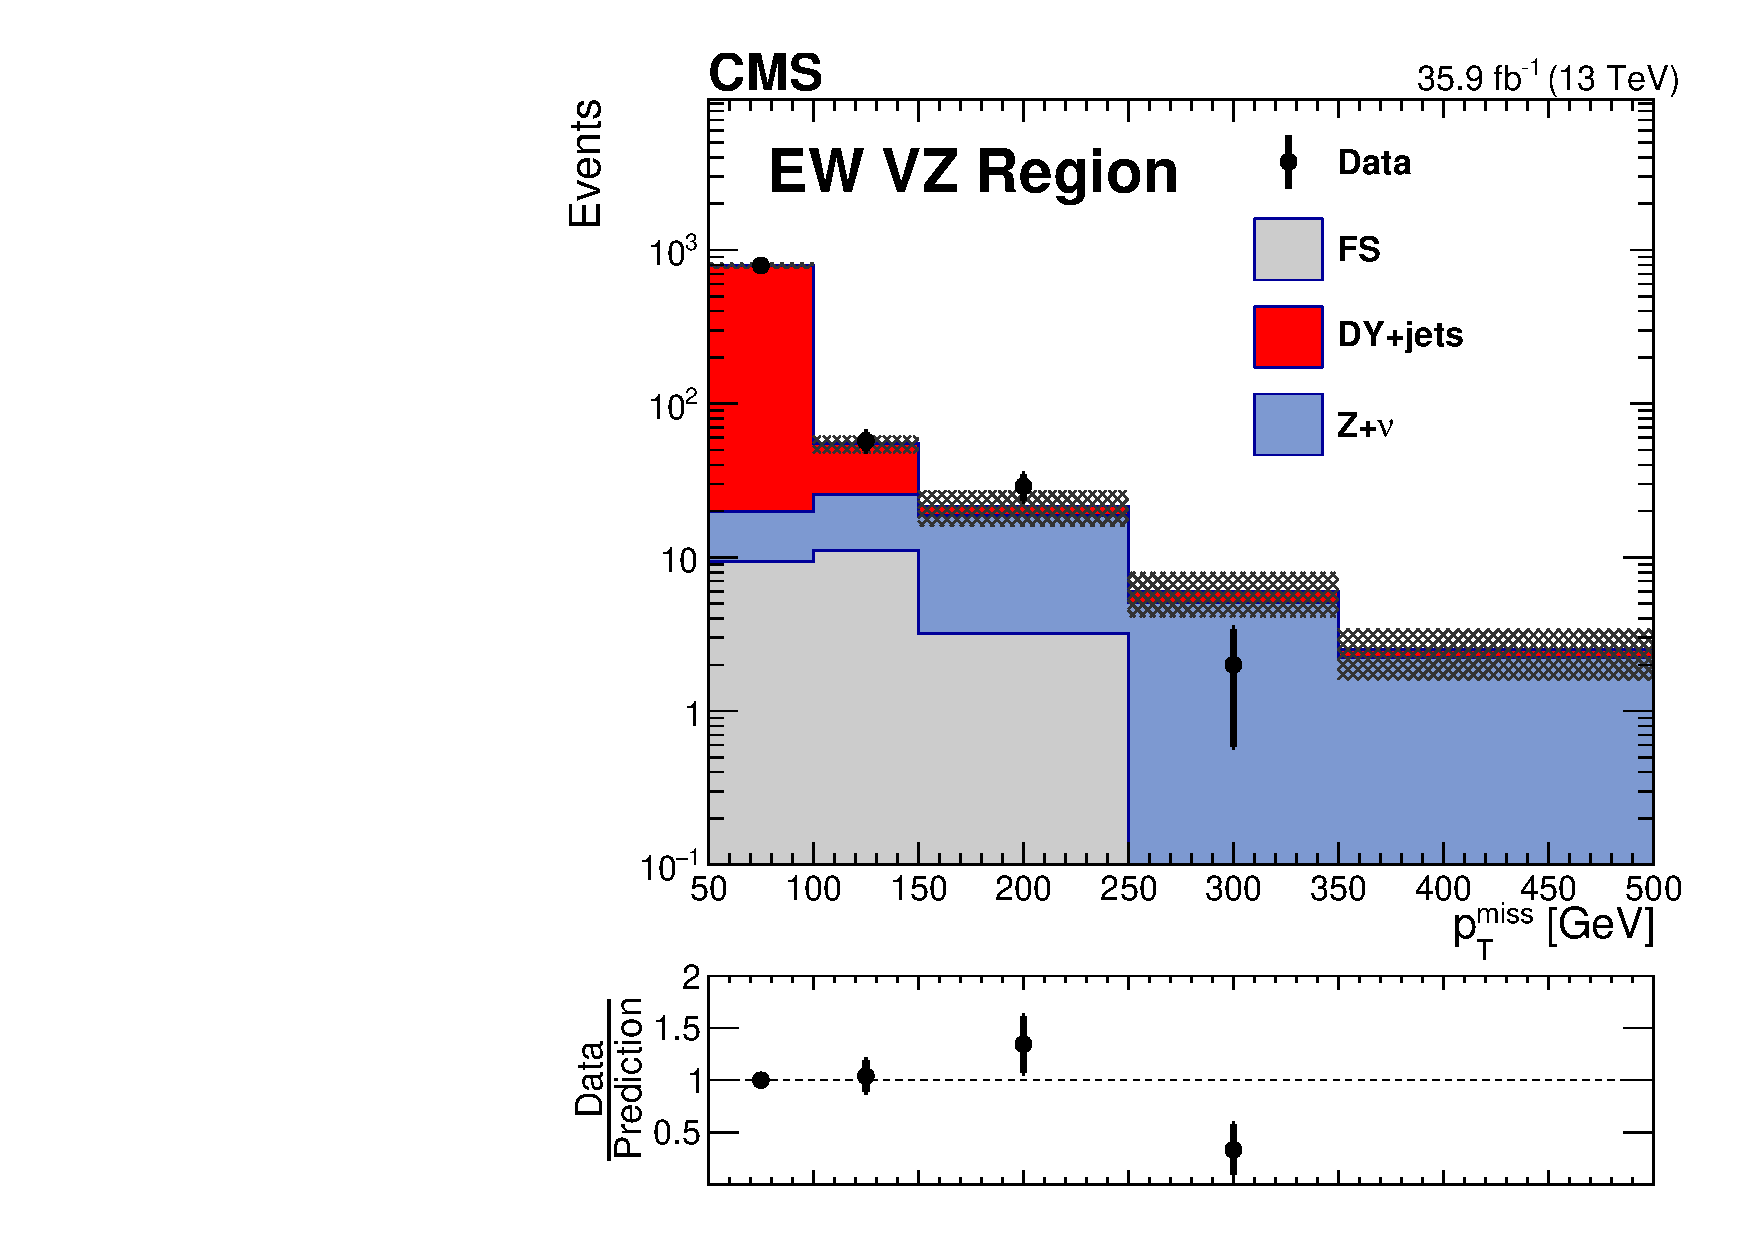
\includegraphics[width=0.4\linewidth]{figures/results/h_met_SR_tcwz.pdf} &
        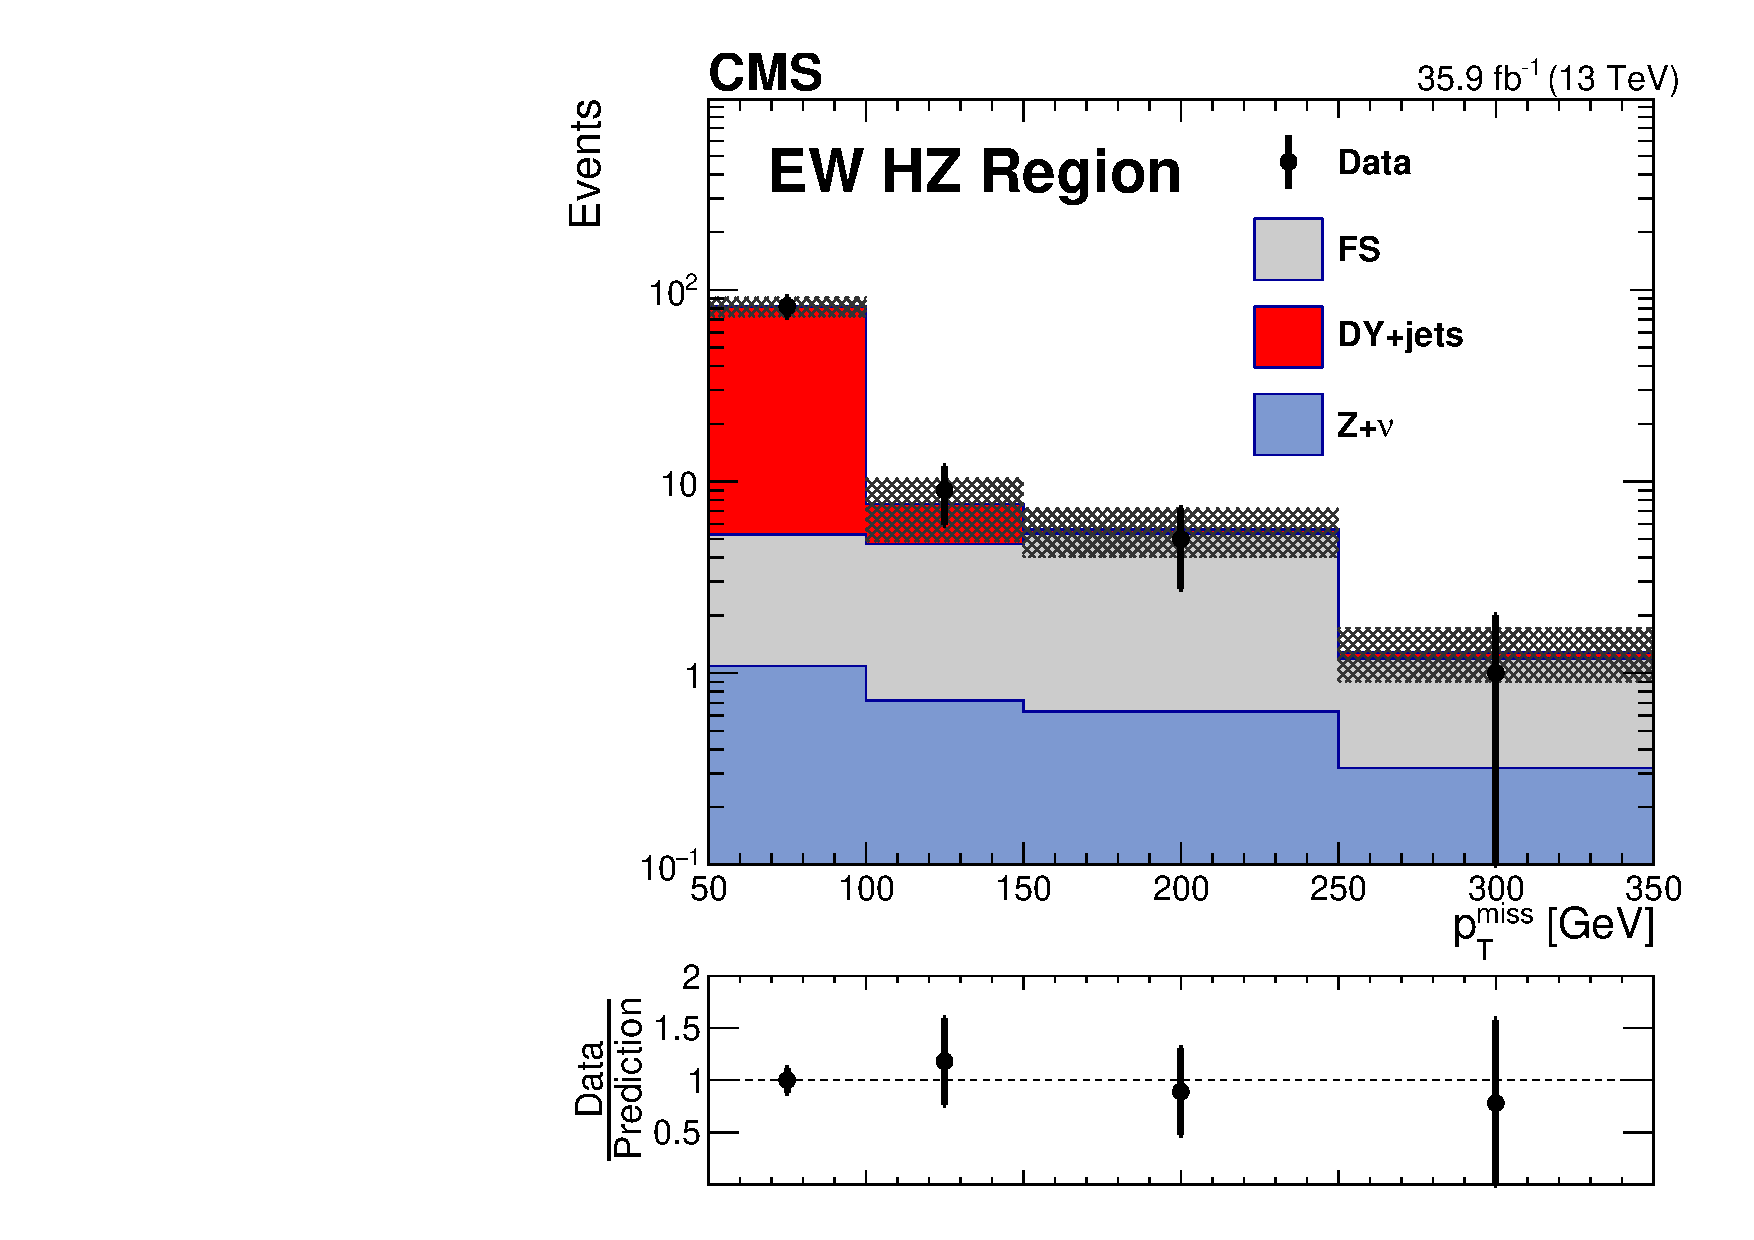
\includegraphics[width=0.4\linewidth]{figures/results/h_met_SR_tchz.pdf} \\
      \end{tabular}
      \caption{\todo{identical cap to AN}
        The \MET\ distribution is shown for data vs. the data-driven predictions in the TChiWZ/ZZ (left), and TChiHZ (right) signal regions. Note that the 50-100 MET bin agrees perfectly by construction as it is used to normalize the DY prediction. See table~\ref{tab:results_SR_ewk}~for yields.
        \label{fig:results_SR_ewk}
      }
    \end{figure}

    \begin{table}[!htb]
      \scriptsize
      \centering
      \caption{\label{tab:results_SR_ewk} \todo{identical cap to AN}
      Results are shown for the electroweak signal regions.
      The uncertainties shown include both statistical and systematic errors. Note that the 50-100 \MET bin agrees perfectly by construction as it is used to normalize the DY prediction. See figure~\ref{fig:results_SR_ewk}~for the corresponding plots.
      }
      \begin{center}
        \begin{tabular} {l | l | l | l | l | l | l }
          TChiWZ & \MET [GeV]  & 50-100 & 100-150 & 150-250 & 250-350 & 350+ \\ \hline 
          & Template  & 773.2$\pm$31.9 & 29.3$\pm$4.4 & 2.9$\pm$2.1 & 1.0$\pm$0.7 & 0.3$\pm$0.3 \\
          & FS  & $9.4^{+3.0}_{-3.0}$  & $11.1^{+3.6}_{-3.6}$  & $3.2^{+1.1}_{-1.1}$  & $0.1^{+0.2}_{-0.1}$  & $0.1^{+0.2}_{-0.1}$  \\
          & Rares  & 10.4$\pm$2.6 & 14.5$\pm$4.0 & 15.5$\pm$5.1 & 5.0$\pm$1.8 & 2.2$\pm$0.9 \\ 
          & Sum  & $793.0^{+32.2}_{-32.2}$  & $54.9^{+7.0}_{-7.0}$  & $21.6^{+5.6}_{-5.6}$  & $6.0^{+1.9}_{-1.9}$  & $2.5^{+0.9}_{-0.9}$ \\ 
          & Data  & 793 & 57 & 29 & 2 & 0 \\ \hline 


          TChiHZ & \MET [GeV]  &  50-100 &  100-150 &  150-250 & \multicolumn{2}{l}{ 250+ } \\ \hline 
          & Template  &  76.7$\pm$9.4 &  2.9$\pm$2.4 &  0.3$\pm$0.2 & \multicolumn{2}{l}{ 0.1$\pm$0.1 } \\ 
          & FS  &  $4.2^{+1.4}_{-1.4}$  &  $4.0^{+1.4}_{-1.4}$  &  $4.7^{+1.6}_{-1.6}$  & \multicolumn{2}{l}{ $0.9^{+0.4}_{-0.4}$  } \\ 
          & Rares  &  1.1$\pm$0.3 &  0.7$\pm$0.2 &  0.6$\pm$0.2 & \multicolumn{2}{l}{ 0.3$\pm$0.1 } \\ 
          & Sum  &  $82.0^{+9.5}_{-9.5}$  &  $7.6^{+2.8}_{-2.8}$  &  $5.6^{+1.6}_{-1.6}$  & \multicolumn{2}{l}{ $1.3^{+0.4}_{-0.4}$ } \\ 
        \end{tabular}
      \end{center}
    \end{table}


    \clearpage

\section{Signal Interpretations} 

  As mentioned previously in \ref{sec:susy_models}, there are several simplified models we use to interpret the search results in the context of electroweak scale supersymmetry. Each signal model has a cross section for production that is set by the masses of the new particles in that model, and we assume that the addition of a process to the standard model only increases the final state counts in sensitive regions (i.e. that there is no negative interference of new physics on the relevant known physics). 

  Events are generated using physics simulation, described in \ref{sec:susy_simulation}, for an interval of \emph{mass points} in each model. Then the compatibility of the observed data are considered under the null-hypothesis and under the hypothesis that the signal model is present in nature. A confidence level is set us using the CL$_s$ method described in \cite{CLS_method}, the details of which are outlined in the next section.

  \subsection{Statistical Treatment}
    This analysis uses the CMS Higgs Combine Tool \cite{higgs_combine} to produce our confidence intervals. A brief description of the statistical methods used are presented in this section, more detail can be found in \cite{higgs_combine}, \cite{Likelihood_Cowen_Cranmer}, and \cite{CLS_method}. 

    In any given search bin, a prediction is made for the expected standard model background as described in \ref{sec:background_estimation_methods}. Each prediction method is characterized by several largely uncorrelated sources of uncertainty, called \emph{nuisance parameters}, whose one $\sigma$ uncertainty bands are combined in quadrature to give a one $\sigma$ band for the background prediction. The set of all such parameters in this analysis is denoted by $\vec{\theta}$. Each nuisance is modeled as a random variable that multiplies the relevant prediction. The distribution from which this random variable is assumed to be sampled is shown in table \ref{tab:systematic_shapes} for every nuisance in this analysis.\footnote{Further details about the uncertainty sources considered for the background predictions can be found in \ref{sec:background_estimation_methods}, and for the signal model prediction in \ref{sec:systematics_in_signal_yield}.}

    \subsubsection{The Likelihood of an Observation}

      The data in any signal bin can be seen as being sampled from a Poisson distribution. Since each search region is independent, the likelihood of observing the results we've seen in data is the product of the likelihoods to see the outcome in each search bin:

      \begin{align} 
        \mathcal{L}(\text{observation}) = \prod_{i \in \text{Search Bin}} \frac{\lambda_i^{n_i} e^{-\lambda_i}}{n_i !}. \label{eq:niave_likelihood}
      \end{align}

      where each $\lambda_i$ and $n_i$ are the expected and observed number of events in search bin $i$ respectively. If the signal does not exists in nature (the background only hypothesis), then $\lambda_i = b$, the background prediction for the bin. If the signal does exist in nature then $\lambda_i = s + b$, the sum of the signal and background predictions\footnote{again, we assume no negative interference}. However, due to the probabilistic nature of the background and signal predictions, $\lambda$ itself must be modeled by a distribution of possible values. 

      \[
        \lambda_i(\vec{\theta}, \mu) = \mu s(\vec{\theta}) + b(\vec{\theta}).
      \]

      We've also added the \emph{signal strength} $\mu$ to the definition of $\lambda$ for later mathematical convenience. $\mu$ is a parameter that allows us to interpolate any further mathematical constructions between the signal+background and null hypothesis by varying from 1 to 0.

      The nuisance parameters are chosen such that they act as multiplicative factors on the prediction value, that is to say for $K$ relevant nuisance parameters\footnote{Not all nuisance parameters effect every prediction. For instance, if $b$ were the prediction of the Z+Hadronic background in SRA, there would be 4 multiplicative factors listed in table \ref{tab:systematic_shapes}} and a central value denoted by $\widetilde{b}$,

      \[
        b(\theta) = \widetilde{b} \times \theta^0 \times ... \times \theta^K,
      \]

      and the same relationship holds for $s(\theta)$. The probability that a nuisance parameter takes a specific value is drawn from a probability distribution that was fit to auxiliary measurements designed to capture the expected variation of the nuisance. The distribution chosen for each nuisance used in this analysis is given in table \ref{tab:systematic_shapes}. 

      Taking into account the probabilistic nature of $\lambda(\vec{\theta}, \mu)$, the likelihood in eq \ref{eq:niave_likelihood} should be updated with a multiplicative factor that accounts for the probability of certain set of values for $\vec{\theta}$. The likelihood that we observe our data given a specific nuisance configuration and signal strength $\mu$

      \begin{equation} 
        \mathcal{L}(\text{observation} | \vec{\theta}, \mu ) = P(\vec{\theta}) \left( \prod_{i \in \text{Search Bin}} \frac{\lambda_i(\vec{\theta}, \mu)^{n_i} e^{-\lambda_i(\vec{\theta}, \mu)}}{n_i !} \right), \label{eq:true_likelihood}
      \end{equation}
      

      where $P(\vec{a})$ is the probability that the nuisance vector has the value $\vec{a}$. Given that we assume the nuisances are completely uncorrelated, $P(\vec{\theta})$ will be a product of terms for each nuisance with distributions chosen from table \ref{tab:systematic_shapes}. As an example, if the only nuisances considered were the luminosity and the closure for the low \MET bin of the SRA Z+Hadronic prediction, where the value of the luminosity multiplicative factor is denoted by $\theta[0]$ and the closure factor is denoted by $\theta[1]$, the full likelihood function for the GMSB signal model would read

      \begin{multline}
          \mathcal{L}(\vec{\theta}, \mu | \text{data} ) = \\
          \underbrace{\frac{1}{\sqrt{2\pi} \ln(1.026)} e^{-\frac{\left(\ln\theta[0]\right)^2}{2 \left(\ln 1.026\right)^2}} \frac{1}{\theta[0]}}_{\text{Log Normal Distribution for Luminosity}} \times \underbrace{\frac{1}{\sqrt{2\pi} \ln(1.2)} e^{-\frac{\left(\ln\theta[1]\right)^2}{2 \left(\ln 1.2\right)^2}} \frac{1}{\theta[1]}}_{\text{Log Normal Distribution for SRA Low \MET Closure}} \times \\
          \underbrace{\frac{\lambda_i(\vec{\theta}, \mu)^{n_{\text{SRA}}} e^{-\lambda_i(\vec{\theta}, \mu)}}{n_{\text{SRA}} !}}_{\text{Poisson Distribution for SRA Bin Count}} \times ... \times \underbrace{\frac{\lambda_i(\vec{\theta}, \mu)^{n_{\text{SRCb}}} e^{-\lambda_i(\vec{\theta}, \mu)}}{n_{\text{SRCb}} !}}_{\text{Only the 6 Strong Search Regions Contribute}}
      \end{multline}


      \todo{the reference cited above is completely incomprehensible. It tries to call $P(\vec{\theta})$ $p(\widetilde{\theta}| \theta) = \frac{p(\theta | \widetilde{\theta})}{\pi_\theta(\theta)}$, but absolutely no definition of those terms is given sans some hand wavy bullshit about it having to do with the probability of having a particular $\theta$ value given the "default value" $\widetilde{\theta}$. It calls $\pi_\theta(\theta)$ hyper-priors as if any motherfucker I have ever met in my 10 years of mathematical interest knows what that means. But what they do not explain at all is how the function is fit to the datacards. }


      \begin{table}[!h]
        \begin{center}
          \footnotesize
          \caption{\label{tab:systematic_shapes} Systematic Uncertainty Assumed Shapes. }
          \begin{tabular}{l | l | l}
            \hline
            \hline
            Prediction  & Nuisance  & Distribution \\
            \hline
            \textbf{Z + Hadronic}     & Closure                    & log Normal \\
                                      & EWK Subtraction            & log Normal \\
                                      & $\gamma$ Normalization     & log Normal \\
                                      & $\gamma$ Statistics        & log Normal \\
            \hline
            \textbf{Flavor Symmetric} & $\kappa$ Value             & log Normal \\
                                      & \rsfof Value               & log Normal \\
                                      & Same Sign Statistics       & $\Gamma$   \\
            \hline
            \textbf{Z + $\nu$}        & Closure                    & log Normal \\
                                      & MC Statistics              & log Normal \\
            \hline
            \textbf{Signal}           & MC Statistics              & log Normal \\
                                      & B-tag eff, heavy flavor    & log Normal \\
                                      & B-tag eff, light flavor    & log Normal \\
                                      & Jet Energy Scale           & log Normal \\
                                      & Lepton Trigger Efficiency  & log Normal \\
                                      & Lepton ID/Iso Efficiency   & log Normal \\
                                      & ISR Modeling               & log Normal \\
                                      & Luminosity                 & log Normal \\
                                      & Fastsim MET Modeling       & log Normal \\
                                      & Generator Scale variations & log Normal \\
                                      & PU reweighting             & log Normal \\
            \hline
            \hline
          \end{tabular}
        \end{center}
      \end{table}
    \subsubsection{The Exclusion Limits}

      In order to exclude a mass point for a signal model, we adopt the CL$_s$ method. The basic premise is that in order for a mass point to be excluded at the 95\% confidence level, we require that, under some metric of probability, that the background only hypothesis is 20 times more likely than the signal+background hypothesis\footnote{$\frac{1}{20}$ being the left of 5\% from 95\%}.

      The metric of probability we use is based upon the following formalism: 

      First, we construct the so-called profile-likelihood ratio, a ``test statistic" defined as

      \begin{align} \label{eq:profile_log_likelihood}
        q_\mu = -2 \ln \left( \frac{\mathcal{L}(\text{observation} | \vec{\theta}_{\mu}, \mu)}{\mathcal{L}(\text{observation} | \vec{\theta}_{\hat{\mu}}, \hat{\mu})} \right)
      \end{align}

      where

      \begin{align*}
        \vec{\theta}_a &= \vec{\theta} \text{ such that } \mathcal{L}(\text{observation} | \vec{\theta}, a) \text{ is maximal, and } \\
        \hat{\mu} &= \mu \text{ such that } \mathcal{L}(\text{observation} | \vec{\theta}_\mu, \mu) \text{ is maximal. \footnotemark{} }
      \end{align*}
      \footnotetext{This means that $\mathcal{L}(\text{observation} | \vec{\theta}_{\hat{\mu}} ,\hat{\mu} )$ is the global maximum of the likelihood}
      
       In the above, we only search over values of $\hat{\mu} \le \mu$, the the global maximum is found outside this region, $q_\mu$ is set to 0. The denominator in eq \ref{eq:profile_log_likelihood} is the global maximum of the likelihood function over all values of $\vec{\theta}$ and $\mu$. The numerator in eq \ref{eq:profile_log_likelihood} is the maximum likelihood of the observed data over all possible $\theta$ configurations, but for a fixed $\mu$. If a value of $\mu$ is very likely, then we expect the $\theta$ parameter to ensure that correlations between bins are not double counted in their effect on the compatibility of the observation. For instance, if the luminosity measurement was 3\% low for our dataset and no new physics exists, the hope is that $\theta_0$ will have the luminosity factor of 1.03.

       Notice that $q_\mu$ is bounded by 0 below and unbounded above. If an observation point is highly likely w.r.t the global maximum, then $q_\mu$ is 0. To define the 95\% confidence interval, it is easiest to think in terms of simulated data. \footnote{ although in practice analytic approximations are made in order to do the following calculations} 

       Let $q^\text{obs}_\mu$ be the value of $q$ for some $\mu$ given the actual results of our experiment shown in \ref{sec:results}. We construct a distribution of the possible values for $q_\mu$ under the null hypothesis by using the likelihood in eq. \ref{eq:true_limits} to give simulated results for an ensemble experiments and compute $q_\mu$ for each simulated result. We assume the distribution of $q_\mu$ to tend larger for larger values of $\mu$ since the probability of measuring a new physics process should decrease with the processes cross section in the null hypothesis, and high values of $q$ are associated with unlikely data. The percentage of simulated experiments where $q_\mu$ is larger than $q^\text{obs}_0$ is called CL$_b$, the ``confidence level" of the background only hypothesis. In short, we compute the percentage of experiments that give a less likely outcome than what we found. \todo{I can't understand why this isn't the percentage lower... None of the papers say lower, so this must be right, but suppose we have perfectly likely data, then $q_0 = 0$. Then our confidence level for the BG only hypothesis is 100\%. I guess this counts up the number of things \emph{less likely} than it. That makes sense actually.}

       We repeat this procedure again, only in this case using the background+signal hypothesis to generate our simulated experiments, i.e. $\mu$ is not required to be 0 in $\lambda$. The percentage of simulated experiments where $q_\mu$ is larger than $q^\text{obs}_\mu$ is called CL$_{s+b}$, the ``confidence level" of the signal+background hypothesis. 

       Finally, the value of $\mu$ for which 

       \[
        \text{CL}_s = \frac{\text{CL}_{s+b}}{\text{CL}_b} \le 0.05
       \]

       is called the exclusion limit for the mass point. If the value of $\mu$ for which this condition met is 1 or more, the mass point can not be excluded at the 95\% level. If the value of $\mu$ is less than 1, then we call the mass point excluded.


  \subsection{Systematics in Signal Yield} \label{sec:systematics_in_signal_yield}
    In order to interpret these results in the context of electroweak scale SUSY, the simplified SUSY models in figure \ref{fig:feynman_str} and \ref{fig:feynman_ewk} are simulated using the madgraph package as explained in sec \ref{sec:susy_simulation}. The simulated events are then run through the same software used to count real data events. 

    The models are 

    The following are the list of nuisance parameters for the expected yields of used when computing the liklihood of the data given the hypothesis that the signal exists. For background we could use these but instead just went with the closure test, also fast-sim shit doesn't exist for the other MC.

    \begin{table}[htb]
      \begin{center}
        \footnotesize
        \caption{\label{tab:syst} Systematic uncertainties of the expected signal yield. }
        \begin{tabular}{l|c}
          \hline
          \hline
          Source                     & Value (\%) \\
          \hline
          MC Statistics              & $\pm$1--60 \\
          B-tag eff, heavy flavor    & $\pm$3    \\
          B-tag eff, light flavor    & $\pm$2    \\
          Jet Energy Scale           & $\pm$1--15  \\
          Lepton Trigger Efficiency  & $\pm$3    \\
          Lepton ID/Iso Efficiency   & $\pm$7    \\
          ISR Modeling               & $\pm$0--7  \\
          Luminosity                 & $\pm$2.6  \\
          Fastsim MET Modeling       & $\pm$1--60    \\
          Generator Scale variations & $\pm$3   \\
          PU reweighting             & $\pm$3    \\
          \hline
          Total uncertainty on signal& $\pm$10--60 \\
          \hline
          \hline
        \end{tabular}
      \end{center}
    \end{table}

    As with all simulated events, there are various ways in which the 

  \subsection{Exclusion Limits}

    In this section, the results in \ref{sec:results} are interpreted in the context of the simplified supersymmetric models described in \ref{sec:susy_models}. For the sake of convenience the Feynman diagrams for these models are reproduced in figure \ref{fig:SUSY_diagrams_interpretation_sec}.

    \begin{figure}[!h]
      \centering
      \begin{subfigure}[b]{0.49\textwidth}
        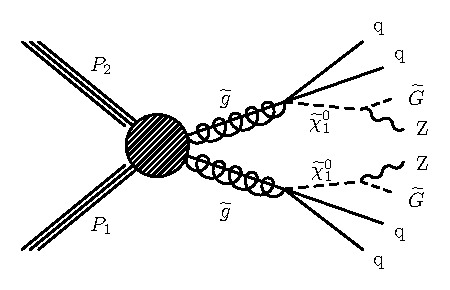
\includegraphics[width=\textwidth]{figures/diagrams/T5ZZ.pdf} 
        \caption{Strong GMSB SUSY}
        \label{fig:t5zz_diagram_interpretations}
      \end{subfigure}
      \begin{subfigure}[b]{0.49\textwidth}
        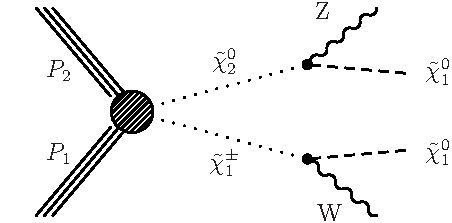
\includegraphics[width=\textwidth]{figures/diagrams/TChiWZ.pdf}
        \caption{EWK SUSY With WZ Production}
        \label{fig:tchiwz_diagram_interpretations}
      \end{subfigure} \\
      \begin{subfigure}[b]{0.49\textwidth}
        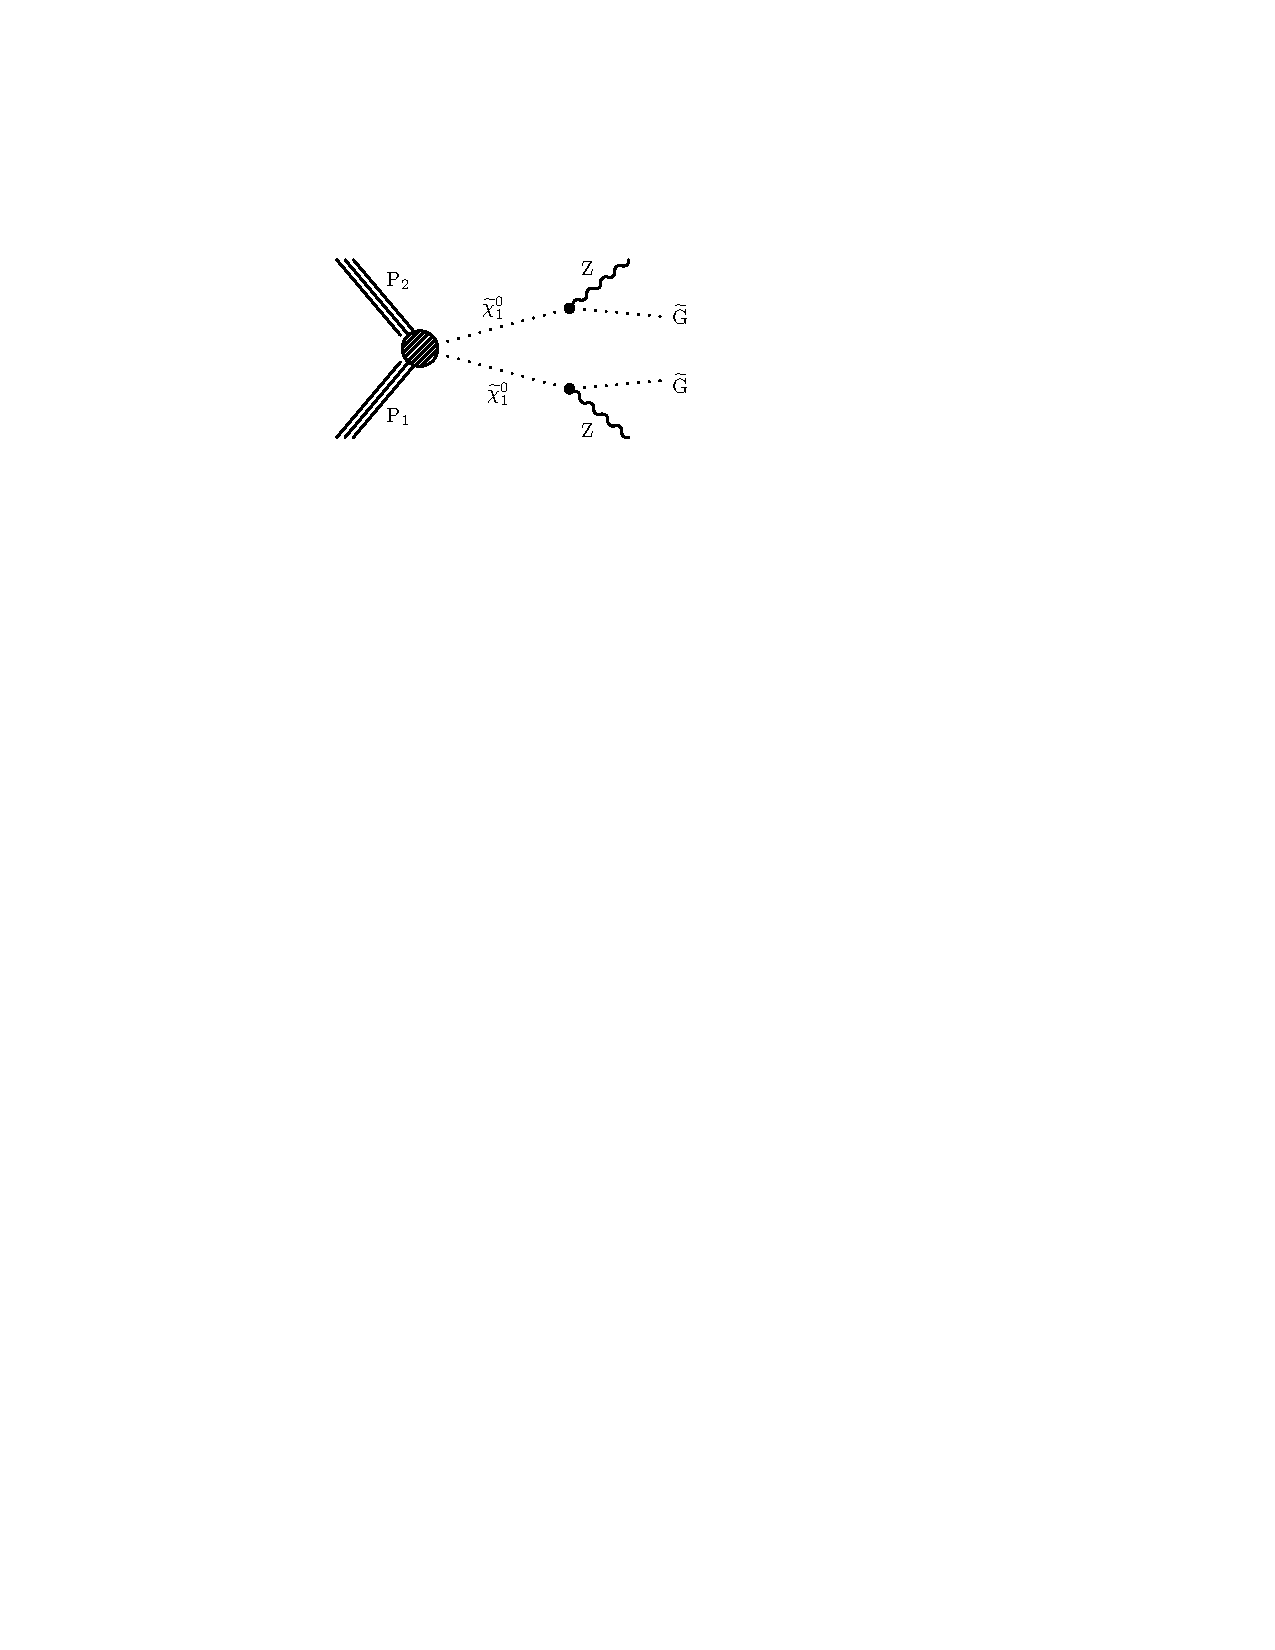
\includegraphics[width=\textwidth]{figures/diagrams/TChiZZ.pdf}
        \caption{EWK SUSY With ZZ Production}
        \label{fig:tchizz_diagram_interpretations}
      \end{subfigure}
      \begin{subfigure}[b]{0.49\textwidth}
        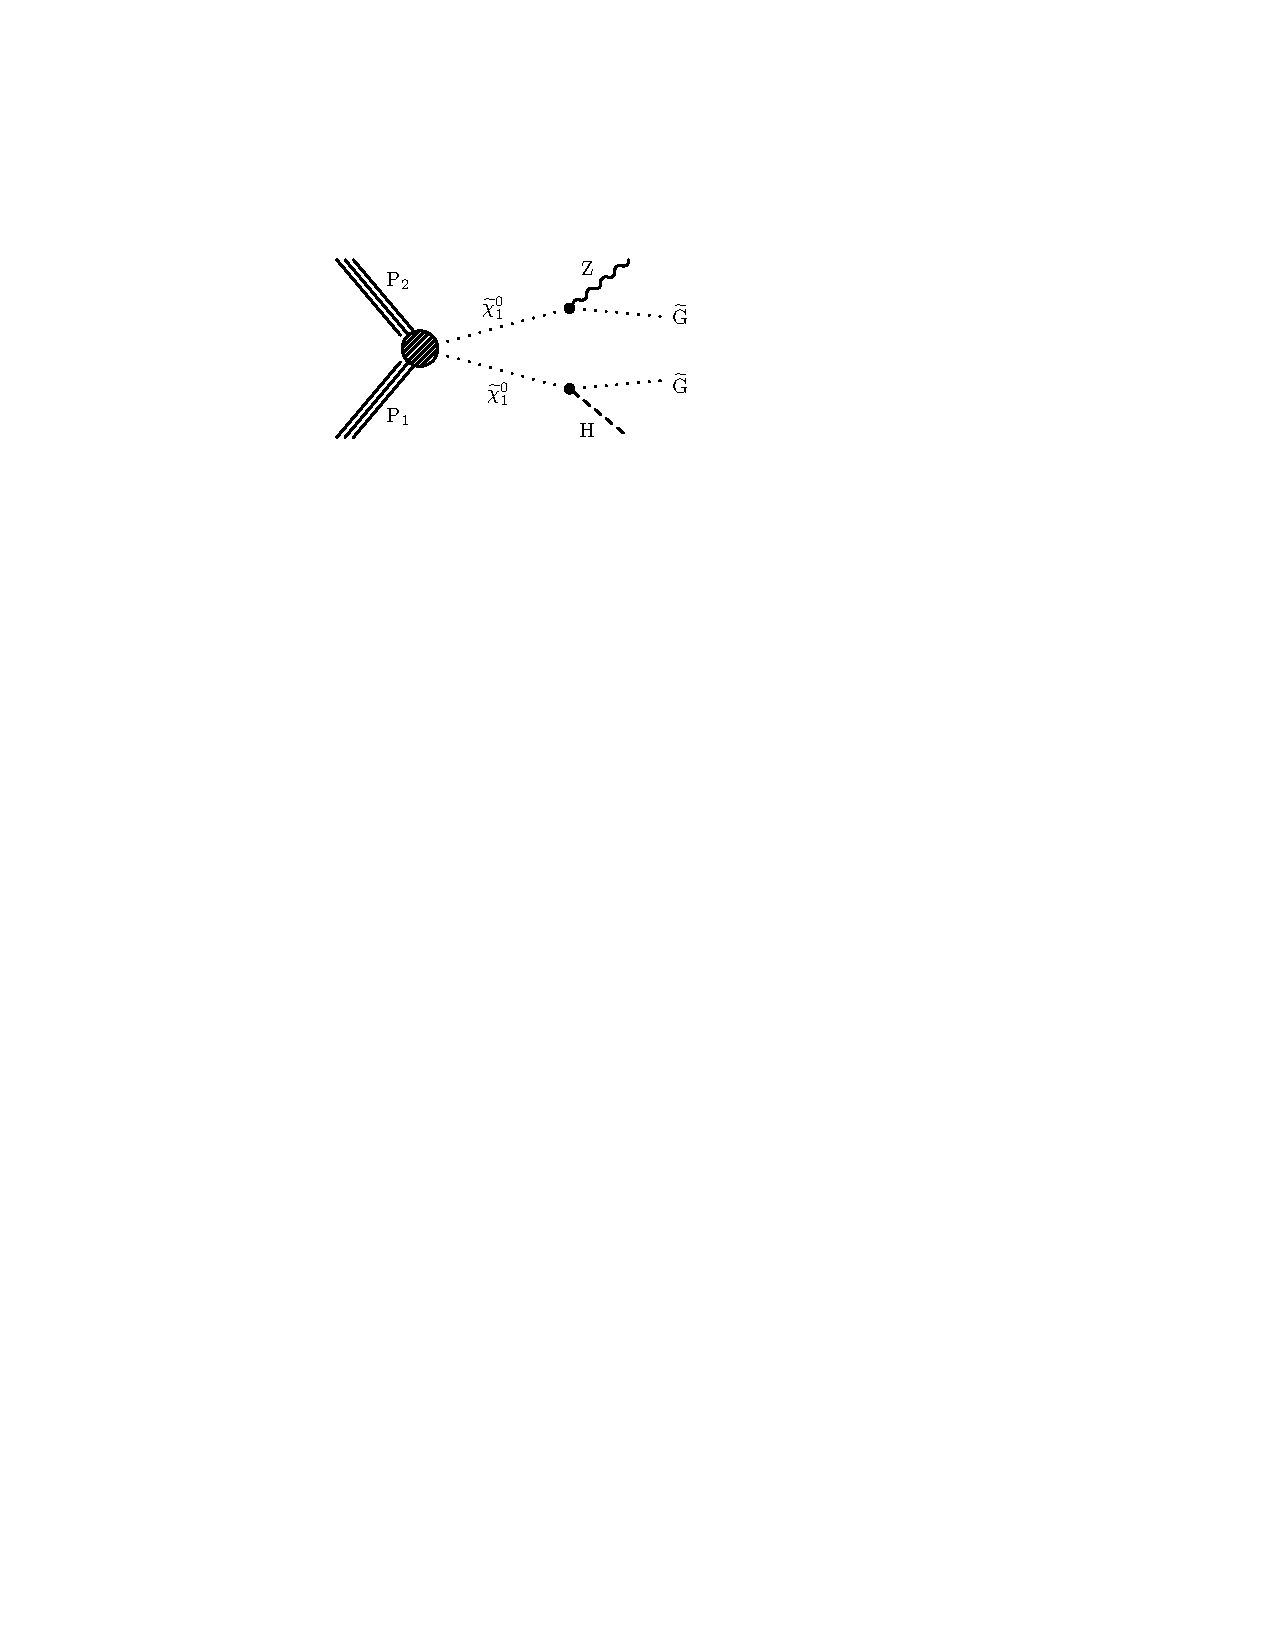
\includegraphics[width=\textwidth]{figures/diagrams/TChiHZ.pdf}
        \caption{EWK SUSY With HZ Production}
        \label{fig:tchihz_diagram_interpretations}
      \end{subfigure}
      \caption{ \label{fig:SUSY_diagrams_interpretation_sec}
        Feynman diagrams for the SUSY models used in interpreting the results of this analysis. More exposition on the properties of these models is found in sec \ref{sec:susy_models}.}
    \end{figure}

    For the strong production model, \ref{fig:t5zz_diagram_interpretations}, the bulk of the sensitivity comes from the high jet multiplicity and high \MET search regions, SRB(b) and SRC(b). In a previous CMS result probing similar final states, this simplified model was excluded at the 95\% CL for gluino masses roughly below 1.2 TeV \cite{paper_2015}. This analysis pushes the limits for the same model by roughly 500 GeV as can be seen in figure \ref{fig:t5zz_interpretation}.

    \begin{figure}[!h]
      \centering
        \begin{subfigure}[b]{0.4\textwidth}
          \label{fig:t5zz_interpretations_2015}
          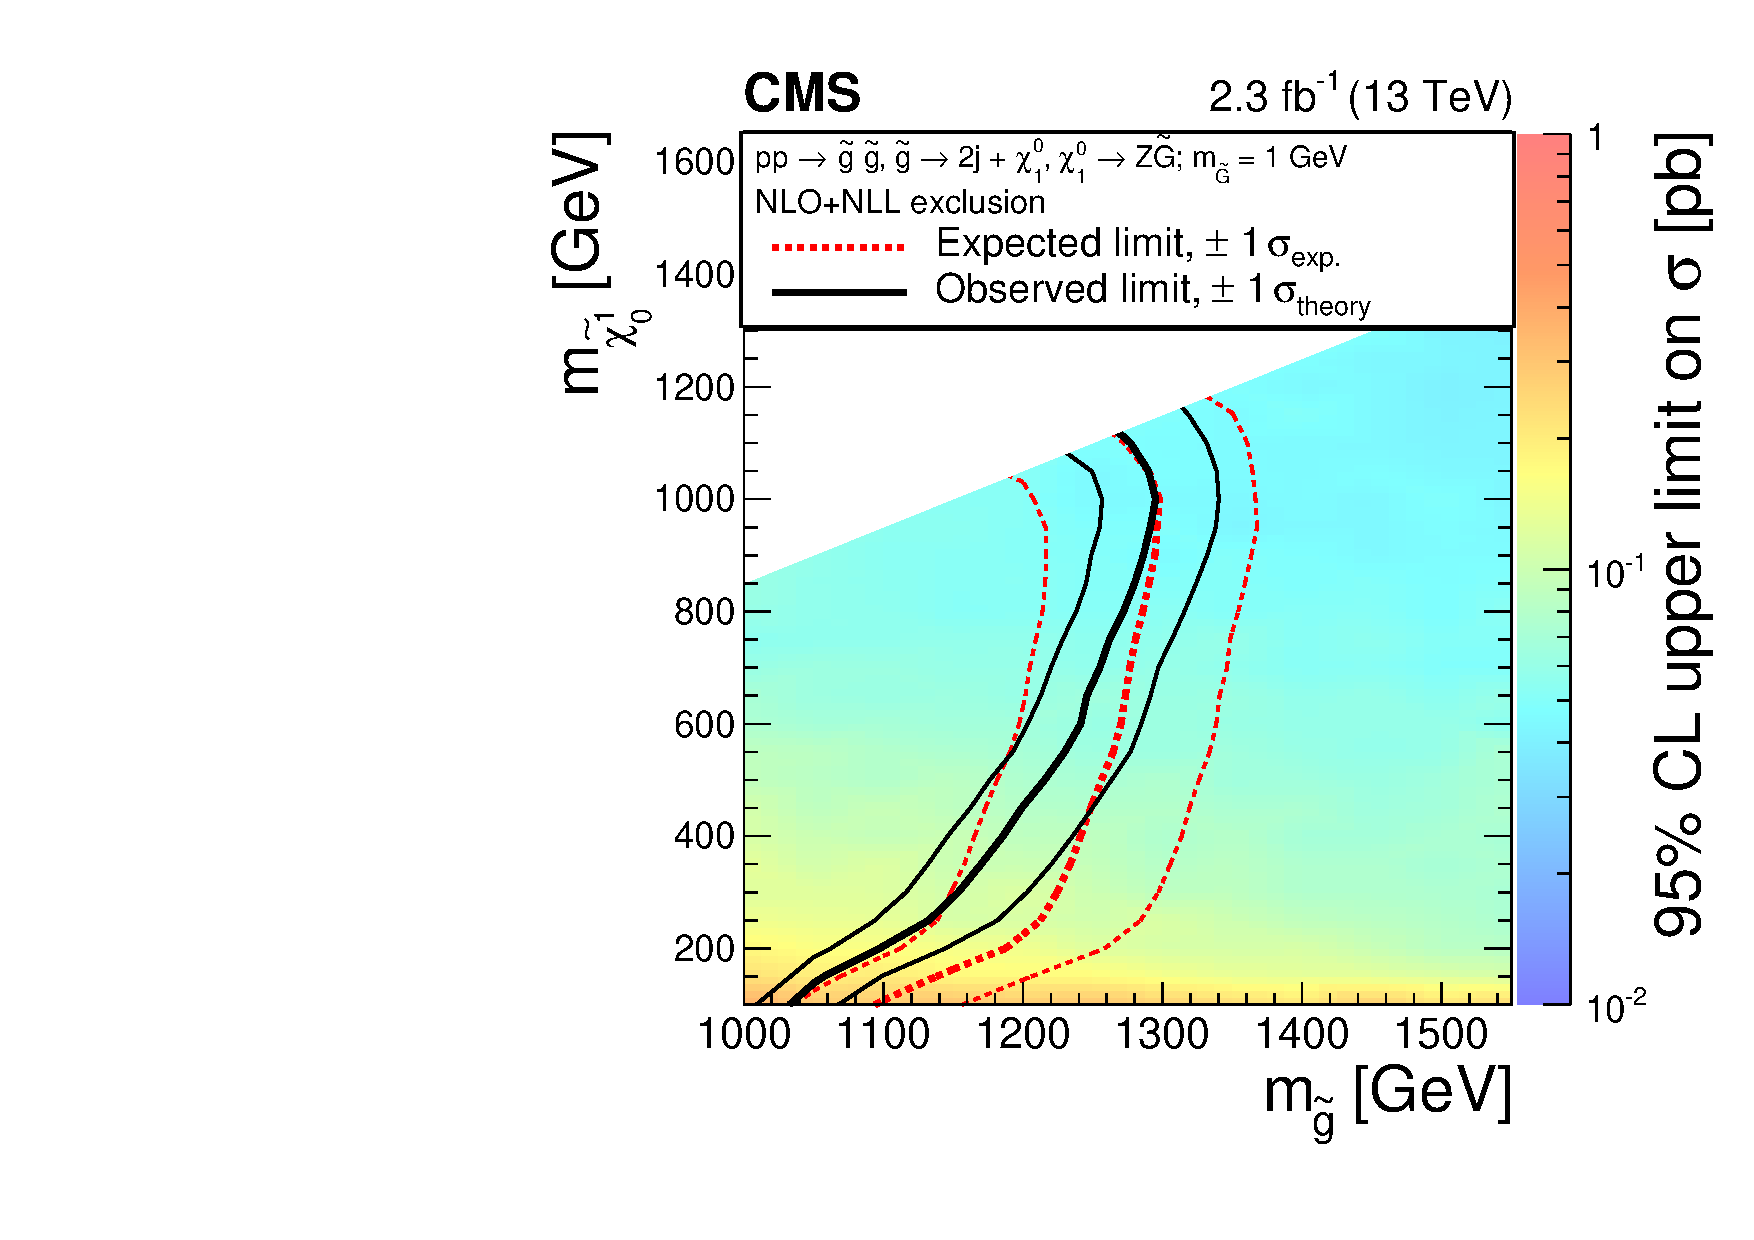
\includegraphics[width=\textwidth]{figures/interpretations/t5zz_2015_exclusion.pdf}
          \caption{Previous best limits on this model}
        \end{subfigure}
        \begin{subfigure}[b]{0.4\textwidth}
          \label{fig:t5zz_interpretations_current}
          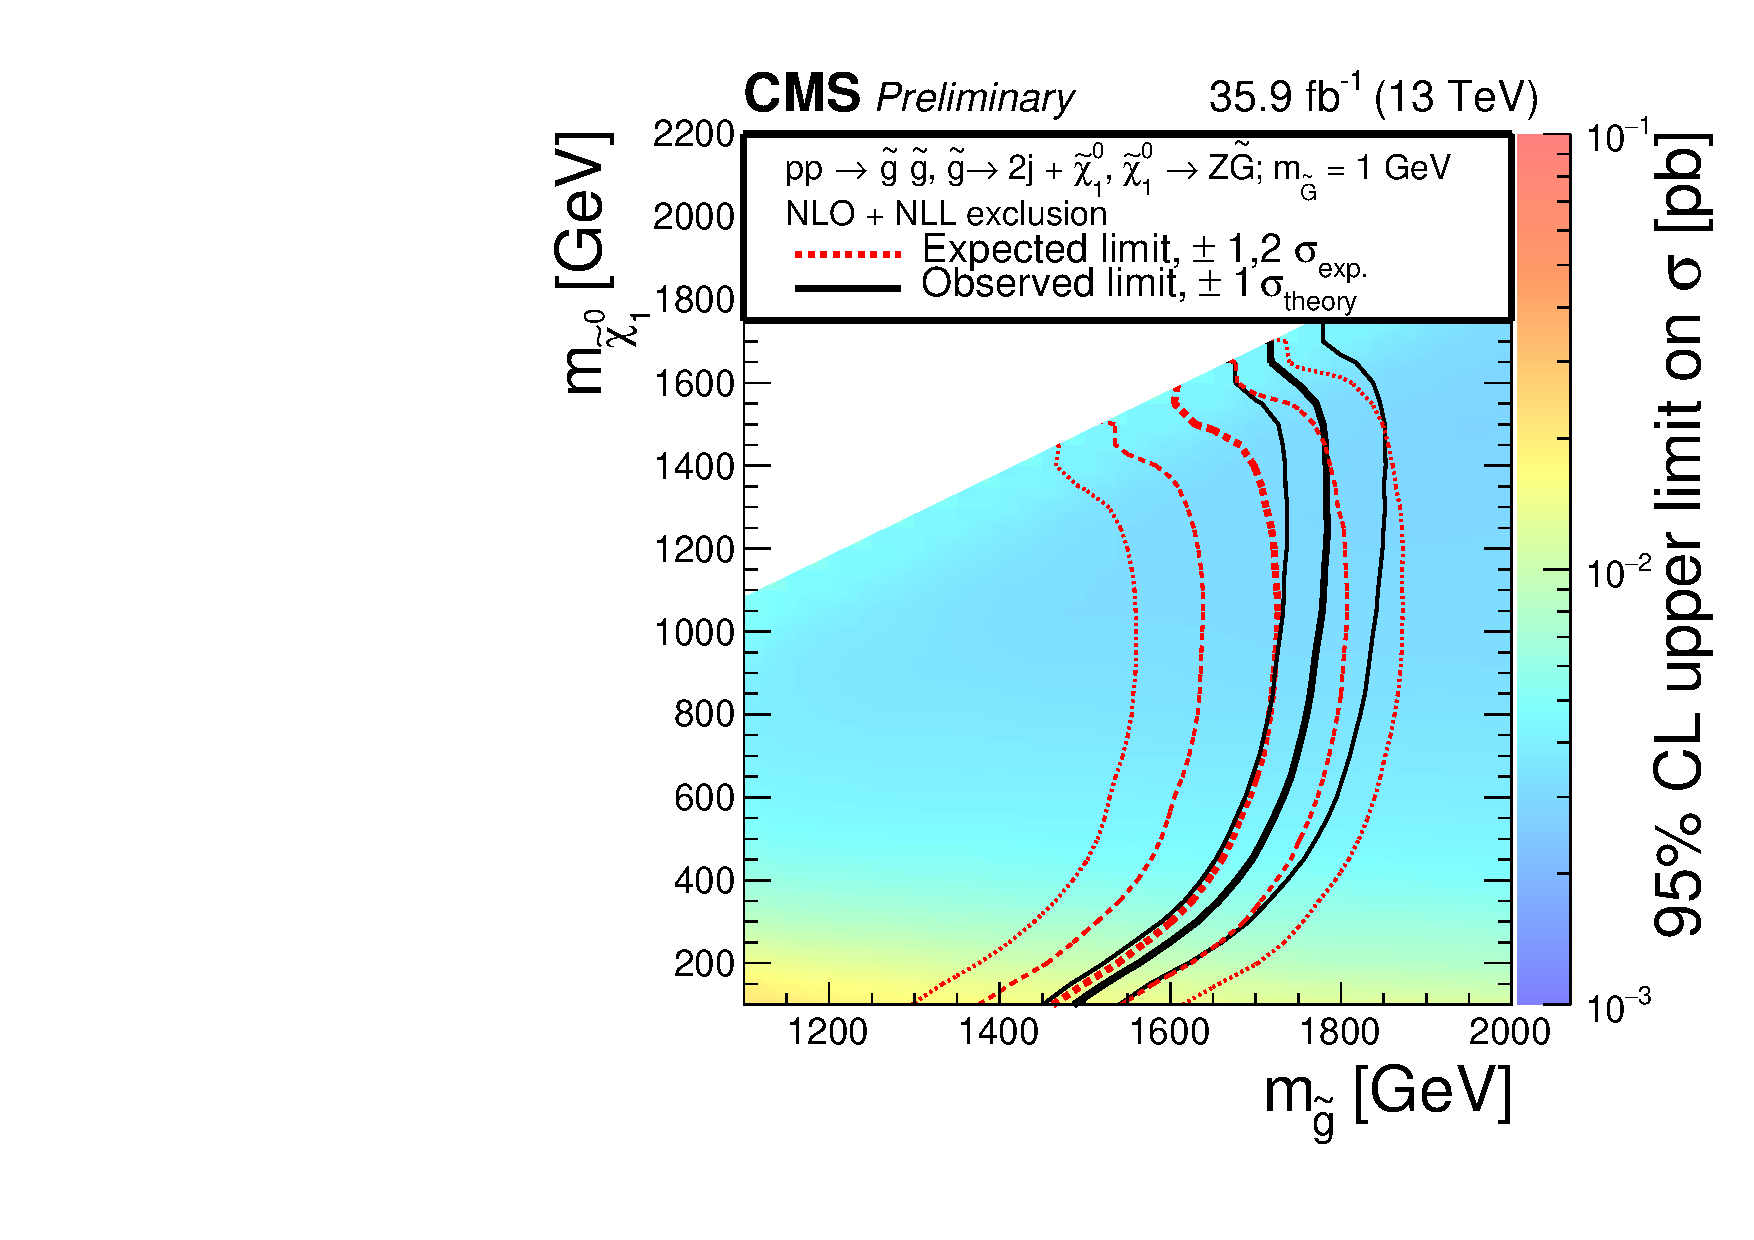
\includegraphics[width=\textwidth]{figures/interpretations/T5ZZ_Exclusion_13TeV.pdf}
          \caption{Limits set by this analysis}
        \end{subfigure}
      \caption{ \label{fig:t5zz_interpretation}
        The limits set on the strong GMSB SUSY model are shown to the right. To the left, we show the previous best limit on this model set by CMS in 2016. This model is excluded at the 95\% CL for gluino masses below 1450 GeV for low LSP masses, and below 1750 GeV for large LSP masses. \todo{check this description: }In the compressed spectrum (where the LSP mass is close to the gluino mass), the LSP is expected to carry away more energy from the gluino than the quarks. In the extremely compressed regions where the LSP and gluino are only separated by a 100 GeV or so of mass, it's possible that one of the jets can be missed. The data shows a downward fluctuation in most of the high \MET bins, except in SRCb, which because of the high jet multiplicity is more sensitive to the uncompressed spectrum. Basically in the high LSP cases, there's some chance for the jets to be lost and that's why the downward fluctuations in SRA and SRB are reflected by creating a better observed limit than the expected one. \todo{ All signal points should all end up in the high MET bin, right? We expect 6 jets normally here because the second Z normally goes to jets. This means that SRC is the most important, yet there is not really a downward fluctuation there. It seems that SRC is related more to the large splitting points and SRA/B are more related to the compressed spectrum... but does the jet argument hold? It seems like in the intermediate mass points we should still expect mostly 6 jet events, yet we already see great space there between the expected and observed limits..}
      }
    \end{figure}

    \begin{figure}[!h]
      \centering
      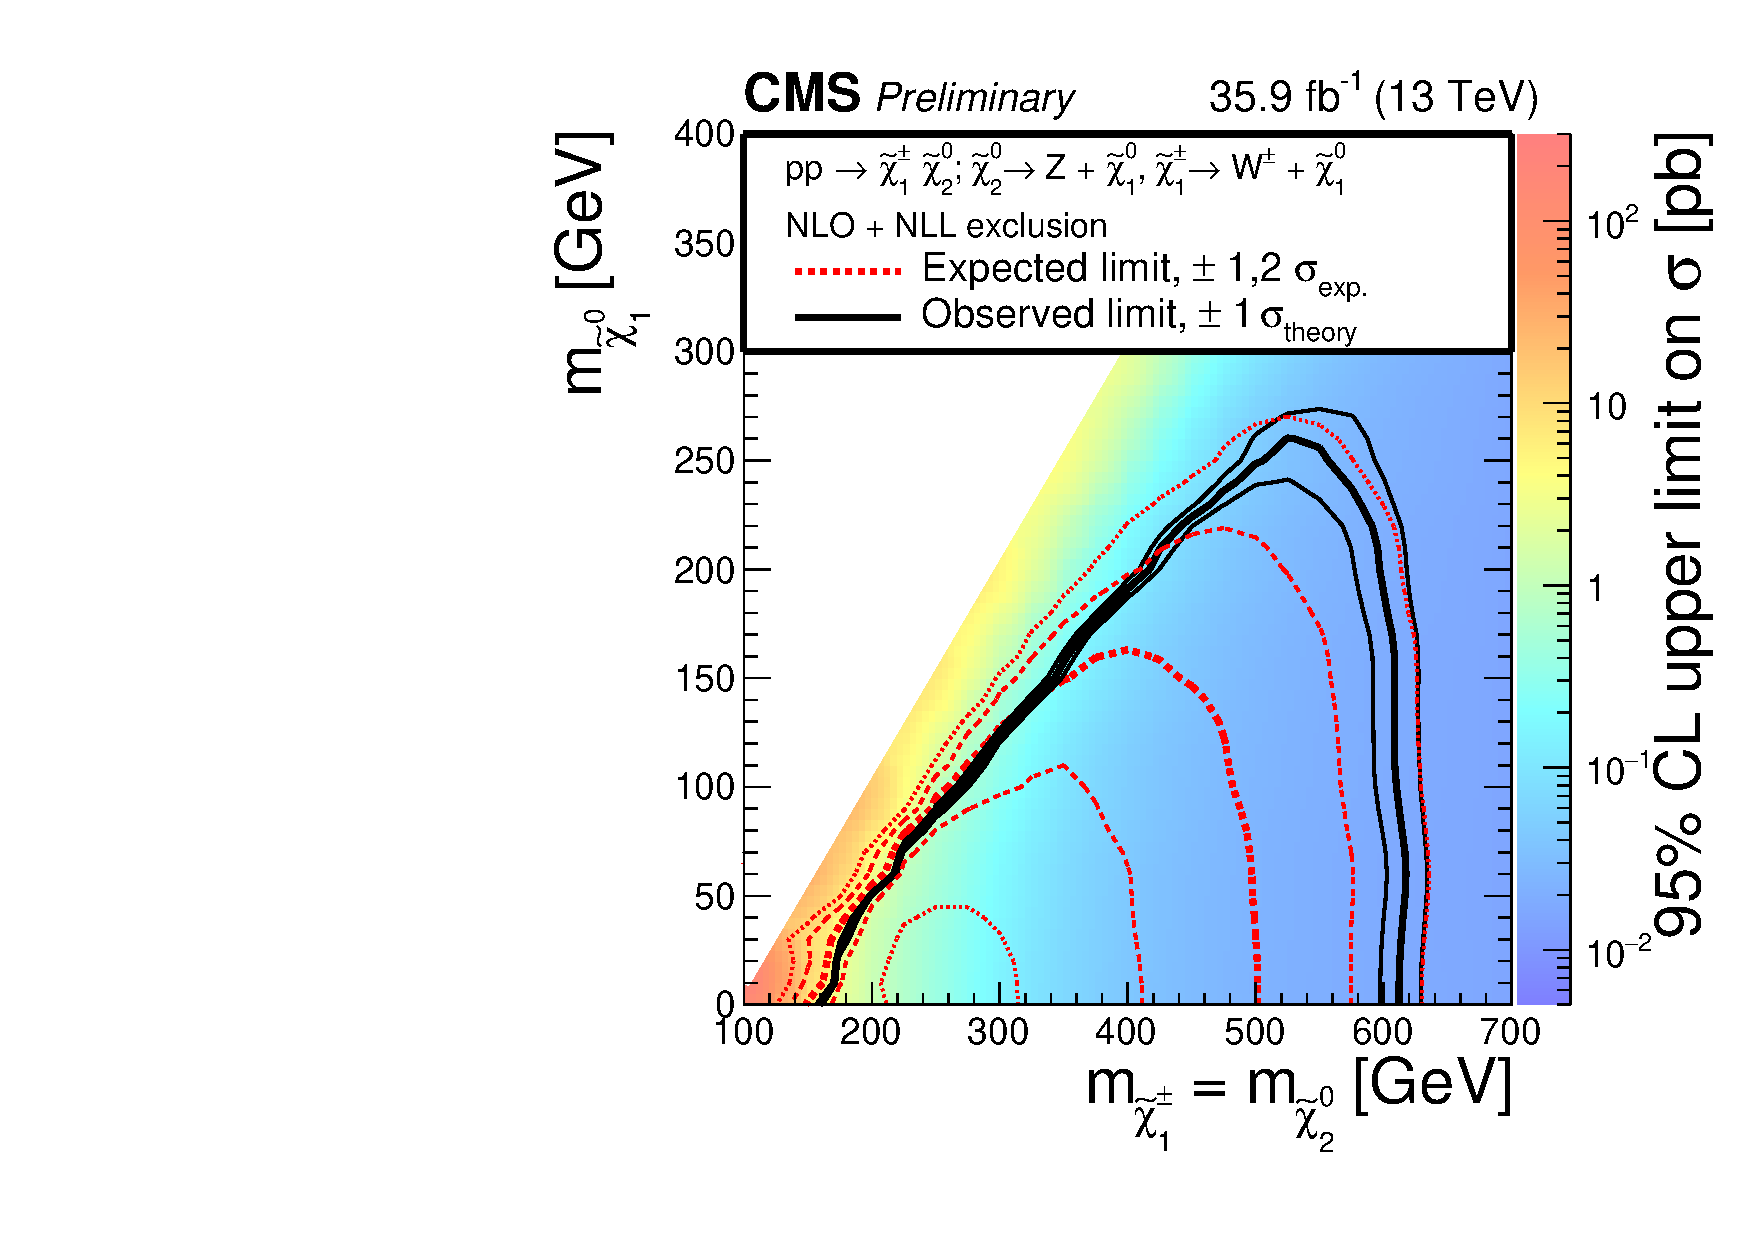
\includegraphics[width=\textwidth]{figures/interpretations/TChiWZ_Exclusion_13TeV.pdf}
      \caption{ \label{fig:tchiwz_interpretation}
        The limits set for the EWK WZ model.
      }
    \end{figure}


    Prior Best T5ZZ Model   -- http://cms-results.web.cern.ch/cms-results/public-results/publications/SUS-15-011/
    Prior Best TChiWZ Model -- http://cms-results.web.cern.ch/cms-results/public-results/publications/SUS-13-006/
    Prior Best TChiZZ Model -- http://cms-results.web.cern.ch/cms-results/public-results/publications/SUS-14-002/
    I think the HZ model is the same as the ZZ model.

\clearpage

\section{The Electroweak Combination}

The things we want to consider here are: 

  1. All the cuts and stuff, I want to list out what cuts we made and why we chose them. I am not sure where I will put all the data/MC agreement stuff. I guess that's mostly important for the MET profile as I don't really use MC in the rest of the
